% Informe del trabajo práctico de Internet de las Cosas (2026/27)
% Basado en la plantilla LLNCS de Springer (samplepaper.tex, v2.20), usada solo por el formato.
%
\documentclass[runningheads]{llncs}
%
\usepackage[T1]{fontenc}
\usepackage[utf8]{inputenc}
\usepackage[spanish,es-tabla,es-nodecimaldot]{babel}
\renewcommand{\andname}{y}  % llncs pone «and» entre autores
\usepackage{graphicx}
\usepackage{xurl}
\usepackage{booktabs}
\usepackage{tabularx}
\usepackage{array}
\usepackage{multirow}
\usepackage{xcolor}
\usepackage{listings}
\usepackage{float}
\usepackage[hidelinks]{hyperref}
\renewcommand\UrlFont{\color{blue}\rmfamily}

\graphicspath{{figuras/}}

% Permitir cortes de línea en identificadores largos (/, _ y ?)
\let\guionbajoorig\_
\AtBeginDocument{\renewcommand{\_}{\guionbajoorig\allowbreak}}
\begingroup\lccode`\~=`\/\lowercase{\endgroup\def~}{\slash}
\AtBeginDocument{\let\urloriginal\url
  \renewcommand{\url}{\begingroup\catcode`\/=12 \urlconbarras}}
\newcommand{\urlconbarras}[1]{\urloriginal{#1}\endgroup}

% --- Código ---------------------------------------------------------------
\definecolor{fondocodigo}{RGB}{247,247,247}
\definecolor{clave}{RGB}{0,90,160}
\definecolor{cadena}{RGB}{163,21,21}
\definecolor{comentario}{RGB}{0,128,0}
\lstset{
  basicstyle=\ttfamily\scriptsize,
  backgroundcolor=\color{fondocodigo},
  frame=single, rulecolor=\color{black!20},
  breaklines=true, breakatwhitespace=false,
  columns=fullflexible, keepspaces=true,
  showstringspaces=false,
  commentstyle=\color{comentario},
  stringstyle=\color{cadena},
  keywordstyle=\color{clave}\bfseries,
  aboveskip=6pt, belowskip=6pt,
  literate={á}{{\'a}}1 {é}{{\'e}}1 {í}{{\'i}}1 {ó}{{\'o}}1 {ú}{{\'u}}1
           {Á}{{\'A}}1 {É}{{\'E}}1 {Í}{{\'I}}1 {Ó}{{\'O}}1 {Ú}{{\'U}}1
           {ñ}{{\~n}}1 {Ñ}{{\~N}}1 {°}{{\textdegree}}1 {→}{{$\rightarrow$}}1
           {…}{{\ldots}}1
}
\lstdefinelanguage{json}{
  string=[s]{"}{"}, comment=[l]{//},
  morekeywords={true,false,null}
}
\lstdefinelanguage{shell}{
  morekeywords={curl,mosquitto_sub,mosquitto_pub,mosquitto,npm,docker,net,cd,node},
  comment=[l]{\#}, string=[b]"
}
\lstdefinelanguage{js}{
  morekeywords={const,let,var,function,return,if,await,new,async},
  comment=[l]{//}, string=[b]'
}

\newcommand{\topic}[1]{\texttt{#1}}
\newcommand{\ruta}[1]{\texttt{#1}}
\newcommand{\pendiente}[1]{\textcolor{red}{\textbf{[#1]}}}

% Tablas con columnas ajustables
\newcolumntype{L}{>{\raggedright\arraybackslash}X}

\begin{document}
\catcode`\/=\active
\sloppy
\setlength{\emergencystretch}{3em}
%
\title{Smart Health: monitorización en tiempo real de la salud de un equipo de fútbol con IoT}
%
\titlerunning{Smart Health: monitorización de futbolistas con IoT}
%
\author{Manuel García Delgado de Mendoza \and Alejandro Sanz Huerta}
%
\authorrunning{M. García Delgado de Mendoza y A. Sanz Huerta}
%
\institute{Internet de las Cosas · Curso 2026/2027\\
Máster en Investigación en Ingeniería de Sistemas y de la Computación\\
Escuela Superior de Ingeniería, Universidad de Cádiz, Cádiz (España)}
%
\maketitle
%
\begin{abstract}
Este trabajo presenta \emph{Smart Health}, una plataforma IoT que vigila en tiempo real la salud de los once jugadores de un equipo de fútbol y avisa al cuerpo médico cuando aparece un riesgo, como un golpe de calor o una frecuencia cardiaca disparada. Cada jugador lleva un \emph{wearable} simulado en Node-RED con seis sensores (GPS, acelerómetro, giroscopio, pulsómetro, termómetro de temperatura interna y plantillas de presión), coordinados por un motor táctico que reproduce un partido en un 4-2-3-1. Las lecturas viajan por MQTT a un broker Mosquitto con usuarios y listas de control de acceso; una pasarela en Node-RED las agrupa en un lote por segundo y las envía a una API REST hecha con Node.js y Express. La API valida los datos, mantiene el estado en vivo de cada jugador, evalúa diez reglas de alerta con umbrales justificados en la literatura, guarda resúmenes en MongoDB y difunde las alertas por MQTT (QoS 1) y por WebSocket. El cuerpo médico trabaja con un \emph{dashboard} web, servido por la propia API, desde el que confirma alertas y fija pautas de readaptación, y con un campograma que muestra a los once jugadores sobre el campo. Como elementos adicionales se incluyen WebSockets, base de datos con colección \emph{time-series}, exposición de constantes vitales en HL7 FHIR R4, documentación OpenAPI con Swagger, una colección de Postman y el control remoto del simulador desde la API.

\keywords{Internet de las Cosas \and MQTT \and Node-RED \and API REST \and Smart Health \and Wearables}
\end{abstract}

%%%%%%%%%%%%%%%%%%%%%%%%%%%%%%%%%%%%%%%%%%%%%%%%%%%%%%%%%%%%%%%%%%%%%%%%%%%%%%
\section{Introducción y motivación}
%%%%%%%%%%%%%%%%%%%%%%%%%%%%%%%%%%%%%%%%%%%%%%%%%%%%%%%%%%%%%%%%%%%%%%%%%%%%%%

Las ciudades inteligentes no son solo tráfico y alumbrado: también incluyen la salud de quienes viven en ellas y las instalaciones donde hacen deporte. En el fútbol, los clubes ya equipan a sus jugadores con dispositivos GPS y pulsómetros, pero esos datos suelen analizarse después del entrenamiento. El riesgo real aparece durante la sesión: un golpe de calor en un partido de verano, una frecuencia cardiaca que no baja tras un esfuerzo o un jugador en readaptación que supera la carga que le permite su lesión.

El objetivo del proyecto es llevar esos datos al cuerpo médico \textbf{en tiempo real}, convertirlos en alertas comprensibles y permitir que el médico actúe sobre ellas. Para ello se integran las tecnologías vistas en la asignatura:

\begin{itemize}
  \item un \textbf{servidor web en Node.js} con una API REST (operaciones GET y POST, además de PUT y DELETE);
  \item un \textbf{broker MQTT} (Mosquitto) por el que viajan las lecturas, las alertas y las órdenes al simulador;
  \item \textbf{varios flujos de Node-RED} que simulan los sensores, hacen de pasarela hacia la API y sirven el \emph{dashboard} médico;
  \item un \textbf{dashboard} médico, un campograma y una botonera de simulación, páginas web servidas por la API que muestran las alertas en tiempo real;
  \item y, como extras, \textbf{WebSockets}, una \textbf{base de datos} MongoDB, el estándar sanitario \textbf{HL7 FHIR}, documentación \textbf{OpenAPI/Swagger} y una colección de \textbf{Postman}.
\end{itemize}

Los datos son simulados, porque no se dispone de \emph{wearables} reales, pero el modelo de simulación es coherente: los seis sensores de cada jugador salen de un único estado de movimiento y los once jugadores se mueven coordinados por un motor táctico.

%%%%%%%%%%%%%%%%%%%%%%%%%%%%%%%%%%%%%%%%%%%%%%%%%%%%%%%%%%%%%%%%%%%%%%%%%%%%%%
\section{Arquitectura del sistema}
%%%%%%%%%%%%%%%%%%%%%%%%%%%%%%%%%%%%%%%%%%%%%%%%%%%%%%%%%%%%%%%%%%%%%%%%%%%%%%

La Fig.~\ref{fig:arquitectura} muestra el sistema completo y el camino que sigue un dato desde el \emph{wearable} simulado hasta el médico. Todo se ejecuta en local: Mosquitto y Node-RED instalados de forma nativa en Windows y MongoDB en un contenedor Docker.

\begin{figure}[!htbp]
\centering
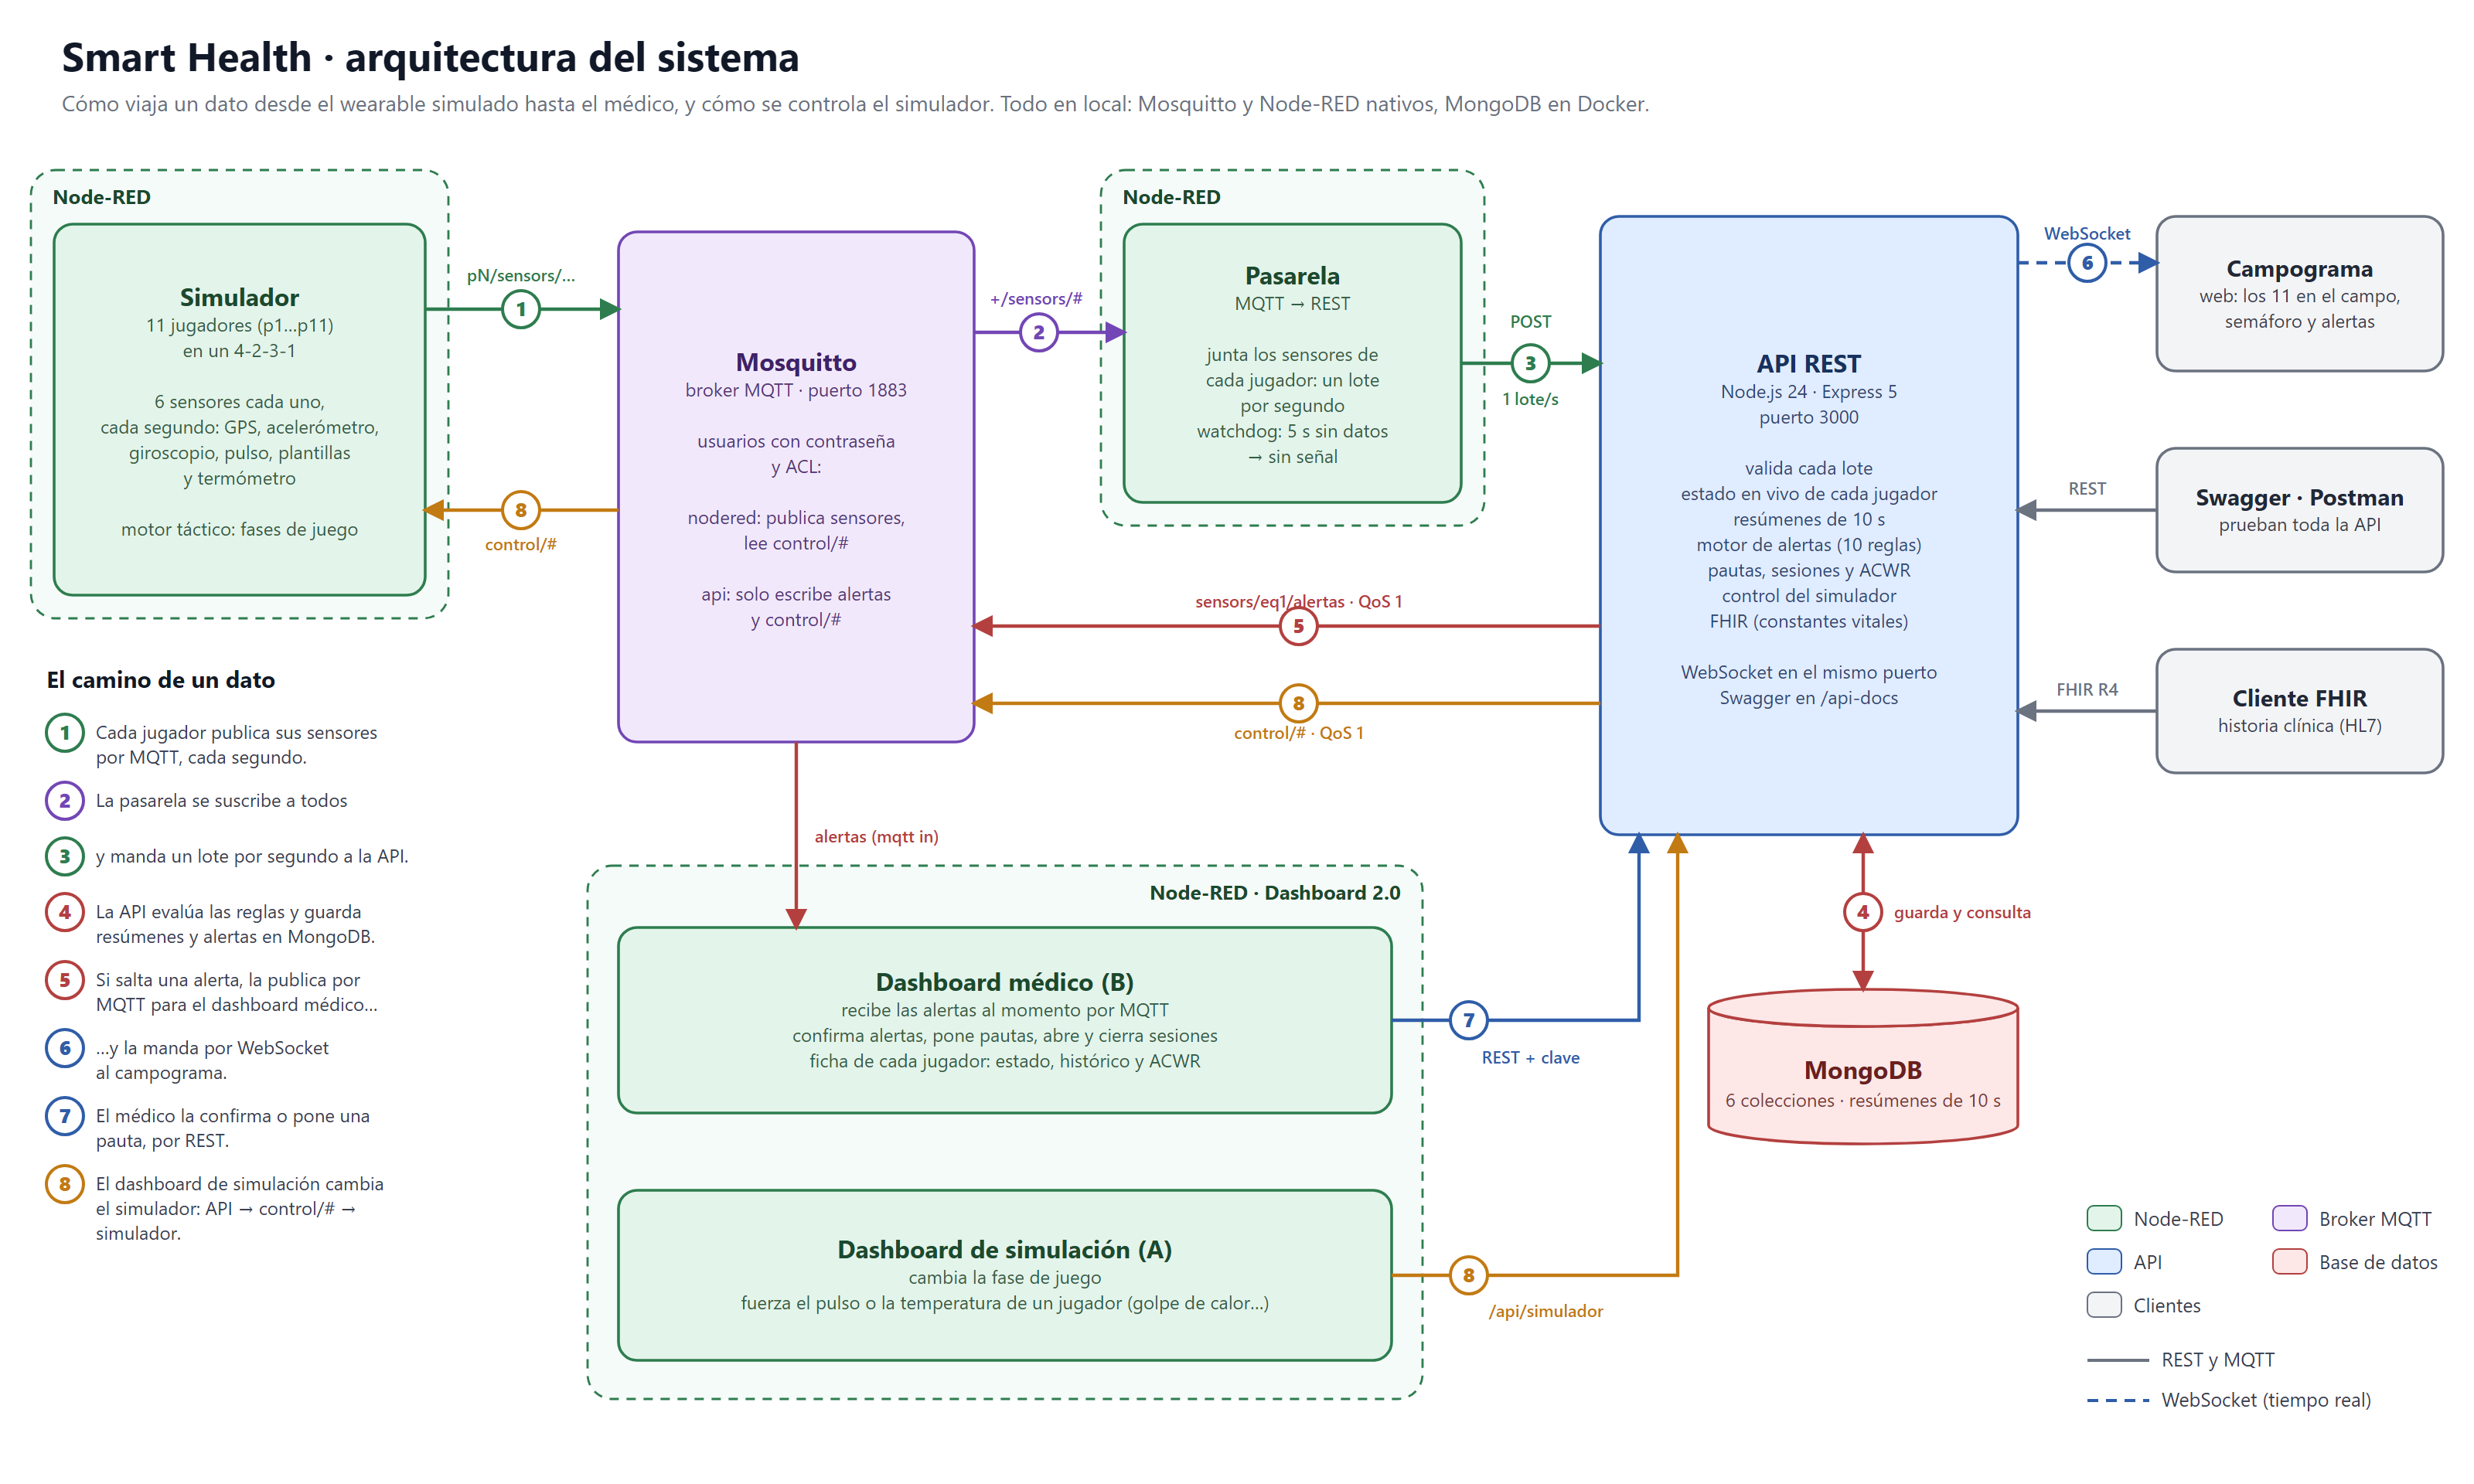
\includegraphics[width=\textwidth]{sistema-arquitectura.png}
\caption{Arquitectura del sistema completo. Los números indican el camino de un dato: (1) cada jugador publica sus sensores por MQTT; (2) la pasarela se suscribe a todos y (3) envía un lote por segundo a la API; (4) la API evalúa las reglas y guarda en MongoDB; (5) publica las alertas por MQTT y (6) las envía por WebSocket al dashboard médico y al campograma; (7) el médico confirma alertas o pone pautas por REST desde su dashboard; (8) la botonera de simulación manda órdenes a la API, que las publica en el broker y de ahí llegan al simulador. El dashboard médico, la botonera y el campograma son páginas web que sirve la propia API.}
\label{fig:arquitectura}
\end{figure}

\subsection{Tecnologías}

\begin{table}[!htbp]
\centering
\caption{Componentes y versiones utilizadas.}\label{tab:tecnologias}
\footnotesize
\begin{tabularx}{\textwidth}{p{3.2cm}p{2.6cm}L}
\toprule
\textbf{Componente} & \textbf{Tecnología} & \textbf{Papel en el sistema} \\
\midrule
Simulador de \emph{wearables} & Node-RED 5 & 11 jugadores, 6 sensores cada uno, publicados a 1~Hz \\
Broker & Mosquitto 2.1 & MQTT 3.1.1 con contraseña y ACL, puerto 1883 \\
Pasarela & Node-RED 5 & MQTT $\rightarrow$ \texttt{POST /api/telemetria}, \emph{watchdog} de 5~s \\
API REST & Node.js 24, Express 5 & Validación, estado en vivo, motor de alertas, puerto 3000 \\
Tiempo real & \texttt{ws} 8 & WebSocket en el mismo puerto que la API \\
MQTT en la API & \texttt{mqtt.js} 5 & Publica alertas y órdenes al simulador (QoS 1) \\
Base de datos & MongoDB 8, Mongoose 9 & 6 colecciones; lecturas en colección \emph{time-series} \\
Dashboard médico & HTML, CSS y JavaScript & Página de la API en \texttt{/medico.html}, con \texttt{fetch} y \texttt{WebSocket} \\
Web & HTML, CSS y JS & Campograma servido por la API en \texttt{/} \\
Documentación & OpenAPI 3.0.3 & Swagger UI en \texttt{/api-docs} y colección de Postman \\
Interoperabilidad & HL7 FHIR R4 & \texttt{Observation} con códigos LOINC y unidades UCUM \\
\bottomrule
\end{tabularx}
\end{table}

\subsection{Decisiones de diseño}

\begin{itemize}
  \item \textbf{La pasarela hace POST en lugar de que Express se suscriba al broker.} Node-RED queda como capa \emph{edge} y la API no depende del formato de cada topic. La pasarela junta los 66 mensajes por segundo en una sola petición, el \emph{watchdog} de ``sin señal'' está donde están los datos y la API se puede probar sin broker (Swagger, Postman).
  \item \textbf{QoS 0 en la telemetría y QoS 1 en las alertas.} Una lectura perdida da igual, porque llega otra al segundo siguiente. Una alerta perdida no: QoS 1 garantiza que llega al menos una vez, y si llega repetida el \emph{dashboard} la identifica por su \texttt{id}. QoS 2 añadiría dos intercambios más que aquí no hacen falta.
  \item \textbf{No se guarda cada mensaje.} Un partido de 90 minutos son 356.400 mensajes MQTT. La API guarda un resumen cada 10~s por jugador (unos 5.940 documentos por partido) y mantiene en memoria el último valor de cada sensor para el tiempo real.
  \item \textbf{El navegador nunca habla con el broker.} Las órdenes al simulador pasan por la API, que las valida y las publica; así el broker sigue cerrado con su ACL y la validación está en un único sitio.
\end{itemize}

%%%%%%%%%%%%%%%%%%%%%%%%%%%%%%%%%%%%%%%%%%%%%%%%%%%%%%%%%%%%%%%%%%%%%%%%%%%%%%
\section{Simulación de los wearables y MQTT}
%%%%%%%%%%%%%%%%%%%%%%%%%%%%%%%%%%%%%%%%%%%%%%%%%%%%%%%%%%%%%%%%%%%%%%%%%%%%%%

\subsection{Motor táctico}

Para que los datos tengan sentido, los once jugadores no se mueven al azar: un nodo \texttt{function} llamado \textbf{MOTOR TÁCTICO} simula un partido en un campo de $105\times68$~m, con el equipo en un 4-2-3-1 que defiende hacia $X=0$ y ataca hacia $X=105$. Cada segundo:

\begin{enumerate}
  \item actualiza la \textbf{fase de juego} con una máquina de estados temporizada: \texttt{ataque\_organizado} (28--40~s), \texttt{transicion\_defensiva} (4~s), \texttt{presion\_alta} (9~s), \texttt{defensa\_organizada} (20~s) y \texttt{transicion\_ofensiva} (6~s);
  \item mueve el \textbf{balón}: con posesión propia lo lleva el poseedor y se intentan pases cada 4--6~s, con preferencia por compañeros adelantados a 7--42~m; con posesión rival, un rival virtual lo empuja hacia nuestra portería;
  \item calcula un \textbf{objetivo} $(X,Y)$ y una velocidad para cada jugador según su rol, la posición del balón y la fase (basculación lateral, línea de centrales, presión de los dos o tres jugadores más cercanos al balón);
  \item envía once órdenes, una por jugador, y publica el estado colectivo en \topic{equipo/estado}.
\end{enumerate}

Las velocidades se limitan por rol: 12~km/h el portero, 25~km/h los defensas, 29~km/h los centrocampistas y 32~km/h los atacantes.

\subsection{Modelo de los seis sensores}

Cada jugador es un nodo \texttt{function} que recibe su orden y calcula, a partir de un único estado de movimiento, sus seis lecturas. Así las medidas de un mismo jugador son coherentes entre sí: si acelera, sube el pulso y, poco a poco, la temperatura.

\begin{table}[!htbp]
\centering
\caption{Sensores simulados de cada jugador.}\label{tab:sensores}
\footnotesize
\begin{tabularx}{\textwidth}{p{2.3cm}p{3.6cm}L}
\toprule
\textbf{Sensor} & \textbf{Medidas} & \textbf{Modelo} \\
\midrule
GPS & velocidad, distancia, posición $X,Y$ & Se mueve hacia su objetivo con aceleración limitada a 2~m/s$^2$ y frenada a 3~m/s$^2$ \\
Acelerómetro & aceleración, desaceleración & Cambio de rapidez en el último segundo, separado en positiva y negativa \\
Giroscopio & cambio de orientación & Giro del vector velocidad, limitado a $\pm90^\circ$ por segundo \\
Pulsómetro & FC (lpm) & Sigue a una carga que depende de la velocidad y la aceleración; sube rápido y baja despacio (60--180~lpm) \\
Termómetro & temperatura interna & Respuesta térmica lenta con la carga (36,2--39,0~$^\circ$C en simulación normal) \\
Plantillas & \% de carga en cada pie & Alternancia de pisada más sesgo lateral y ruido; ambos pies suman 100~\% \\
\bottomrule
\end{tabularx}
\end{table}

\subsection{Topics y payloads}

Cada jugador publica cada segundo en \topic{<jugador>/sensors/<sensor>}, con identificadores seudónimos \texttt{p1}\ldots\texttt{p11}. Cada medida tiene la forma \texttt{\{unit, value\}}:

\begin{lstlisting}[language=json]
p8/sensors/gps            {"speed":{"unit":"km/h","value":28.7},"distancecovered":{"unit":"m","value":7842},
                           "position":{"X":{"unit":"m","value":52.3},"Y":{"unit":"m","value":30.1}}}
p8/sensors/accelerometer  {"acceleration":{"unit":"m/s2","value":1.25},"desacceleration":{"unit":"m/s2","value":0}}
p8/sensors/giroscope      {"changeinposition":{"unit":"degrees","value":-25.6}}
p8/sensors/pulsemeter     {"pulse":{"unit":"bpm","value":181}}
p8/sensors/pressuresensor {"pressureleftfoot":{"unit":"%","value":42},"pressurerightfoot":{"unit":"%","value":58}}
p8/sensors/thermometer    {"temperature":{"unit":"C","value":38.2}}
\end{lstlisting}

\begin{table}[!htbp]
\centering
\caption{Topics MQTT del sistema.}\label{tab:topics}
\footnotesize
\begin{tabularx}{\textwidth}{p{4.2cm}p{1.9cm}p{0.8cm}L}
\toprule
\textbf{Topic} & \textbf{Publica} & \textbf{QoS} & \textbf{Contenido} \\
\midrule
\topic{pN/sensors/<sensor>} & Simulador & 0 & Lectura de un sensor, 1~Hz por sensor \\
\topic{equipo/estado} & Simulador & 0 & Fase, posesión, balón y objetivos tácticos \\
\topic{sensors/eq1/alertas} & API & 1 & Alerta completa, para el \emph{dashboard} médico \\
\topic{control/fase} & API & 1 & Nueva fase de juego \\
\topic{control/jugadores/<id>/sensores} & API & 1 & Forzar el pulso o la temperatura de un jugador \\
\topic{control/reset} & API & 1 & Volver a la formación inicial \\
\bottomrule
\end{tabularx}
\end{table}

Con el reloj a 1~Hz, el simulador publica $11\times6+1=67$ mensajes por segundo, unos 241.200 por hora.

\subsection{Mosquitto: usuarios y ACL}

El Mosquitto del proyecto se lanza con su propia configuración (\ruta{mosquitto/mosquitto.conf}), que \textbf{no admite conexiones anónimas} y aplica una lista de control de acceso con mínimo privilegio:

\begin{lstlisting}[language=shell]
# mosquitto.conf
listener 1883
allow_anonymous false
password_file mosquitto/passwd
acl_file mosquitto/acl

# acl: Node-RED (simulador, pasarela y dashboard)
user nodered
topic readwrite sensors/#
topic readwrite +/sensors/#
topic readwrite equipo/#
topic read control/#
# acl: la API solo publica alertas y órdenes al simulador
user api
topic write sensors/+/alertas
topic write control/#
\end{lstlisting}

El fichero \texttt{passwd} guarda las contraseñas con \emph{hash} (\texttt{mosquitto\_passwd}) y no se sube al repositorio. La Fig.~\ref{fig:mosquitto} muestra el tráfico real del broker visto con \texttt{mosquitto\_sub} y el usuario \texttt{nodered}.

\begin{figure}[!htbp]
\centering
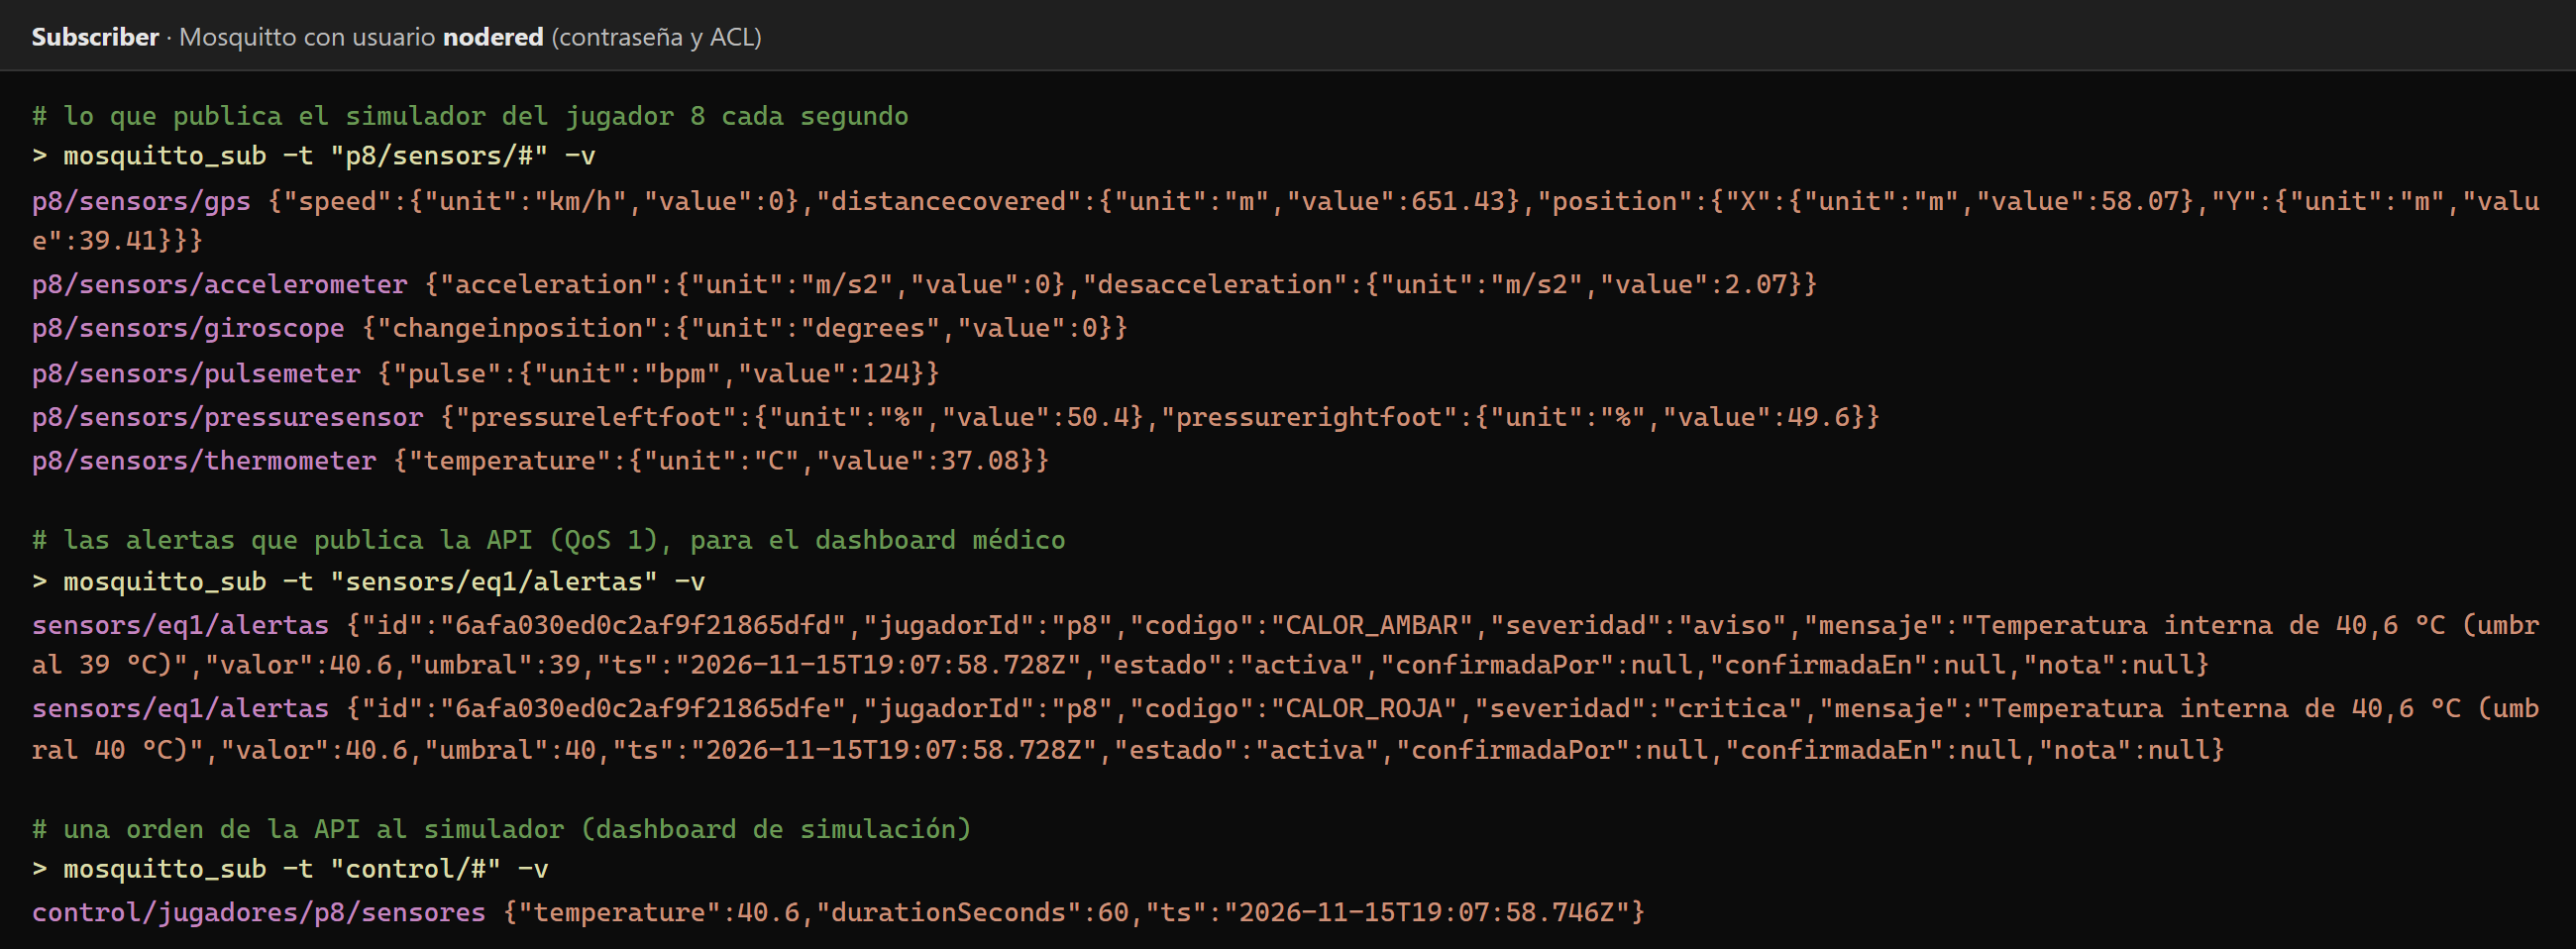
\includegraphics[width=\textwidth]{mosquitto-sub.png}
\caption{El broker por dentro: los seis sensores que publica p8 cada segundo, las dos alertas de calor que publica la API con QoS 1 y la orden que la API envía al simulador.}
\label{fig:mosquitto}
\end{figure}

\subsection{Control del simulador por MQTT}

Para la demostración hay que poder provocar un golpe de calor o una FC disparada cuando se quiera, sin tocar Node-RED. El camino es el inverso al de la telemetría: \textbf{la API publica y el simulador se suscribe}.

\begin{enumerate}
  \item La botonera de simulación (Sección~\ref{sec:botonera}), Swagger o Postman llaman a \texttt{PUT /api/simulador/jugadores/p8/sensores} con \texttt{\{"temperature": 40.5, "durationSeconds": 60\}}.
  \item La API valida la orden y la publica con QoS 1 en \topic{control/jugadores/p8/sensores}.
  \item En el simulador, un \texttt{mqtt in} recibe la orden y el nodo \emph{Guardar ajustes de sensores} la guarda en el contexto del flujo.
  \item El nodo \emph{Aplicar ajustes de sensores} intercepta lo que publica cada jugador y sustituye solo el valor ajustado: durante 60~s p8 publica 40,5~$^\circ$C; el resto de sus sensores y los otros diez jugadores siguen igual.
  \item La telemetría vuelve por el camino normal y saltan \texttt{CALOR\_AMBAR} y \texttt{CALOR\_ROJA}.
\end{enumerate}

Se fuerza la lectura y no el estado interno del jugador para no tocar las funciones de los once jugadores ni el motor táctico. Los rangos permitidos (30--220~lpm y 35--42~$^\circ$C) caben en la validación de la API y permiten provocar las alertas: con el máximo normal de 39~$^\circ$C nunca saltaría \texttt{CALOR\_ROJA}.

%%%%%%%%%%%%%%%%%%%%%%%%%%%%%%%%%%%%%%%%%%%%%%%%%%%%%%%%%%%%%%%%%%%%%%%%%%%%%%
\section{Flujos de Node-RED}
%%%%%%%%%%%%%%%%%%%%%%%%%%%%%%%%%%%%%%%%%%%%%%%%%%%%%%%%%%%%%%%%%%%%%%%%%%%%%%

El proyecto tiene dos flujos (pestañas) en el mismo Node-RED. Las credenciales del broker no aparecen en los nodos: se leen del \texttt{.env} mediante \texttt{\$\{NODERED\_MQTT\_USER\}} y \texttt{\$\{NODERED\_MQTT\_PASS\}} al arrancar con \ruta{node\_red/arrancar.js}.

\subsection{Flujo \emph{Jugadores}: el simulador}

\begin{figure}[!htbp]
\centering
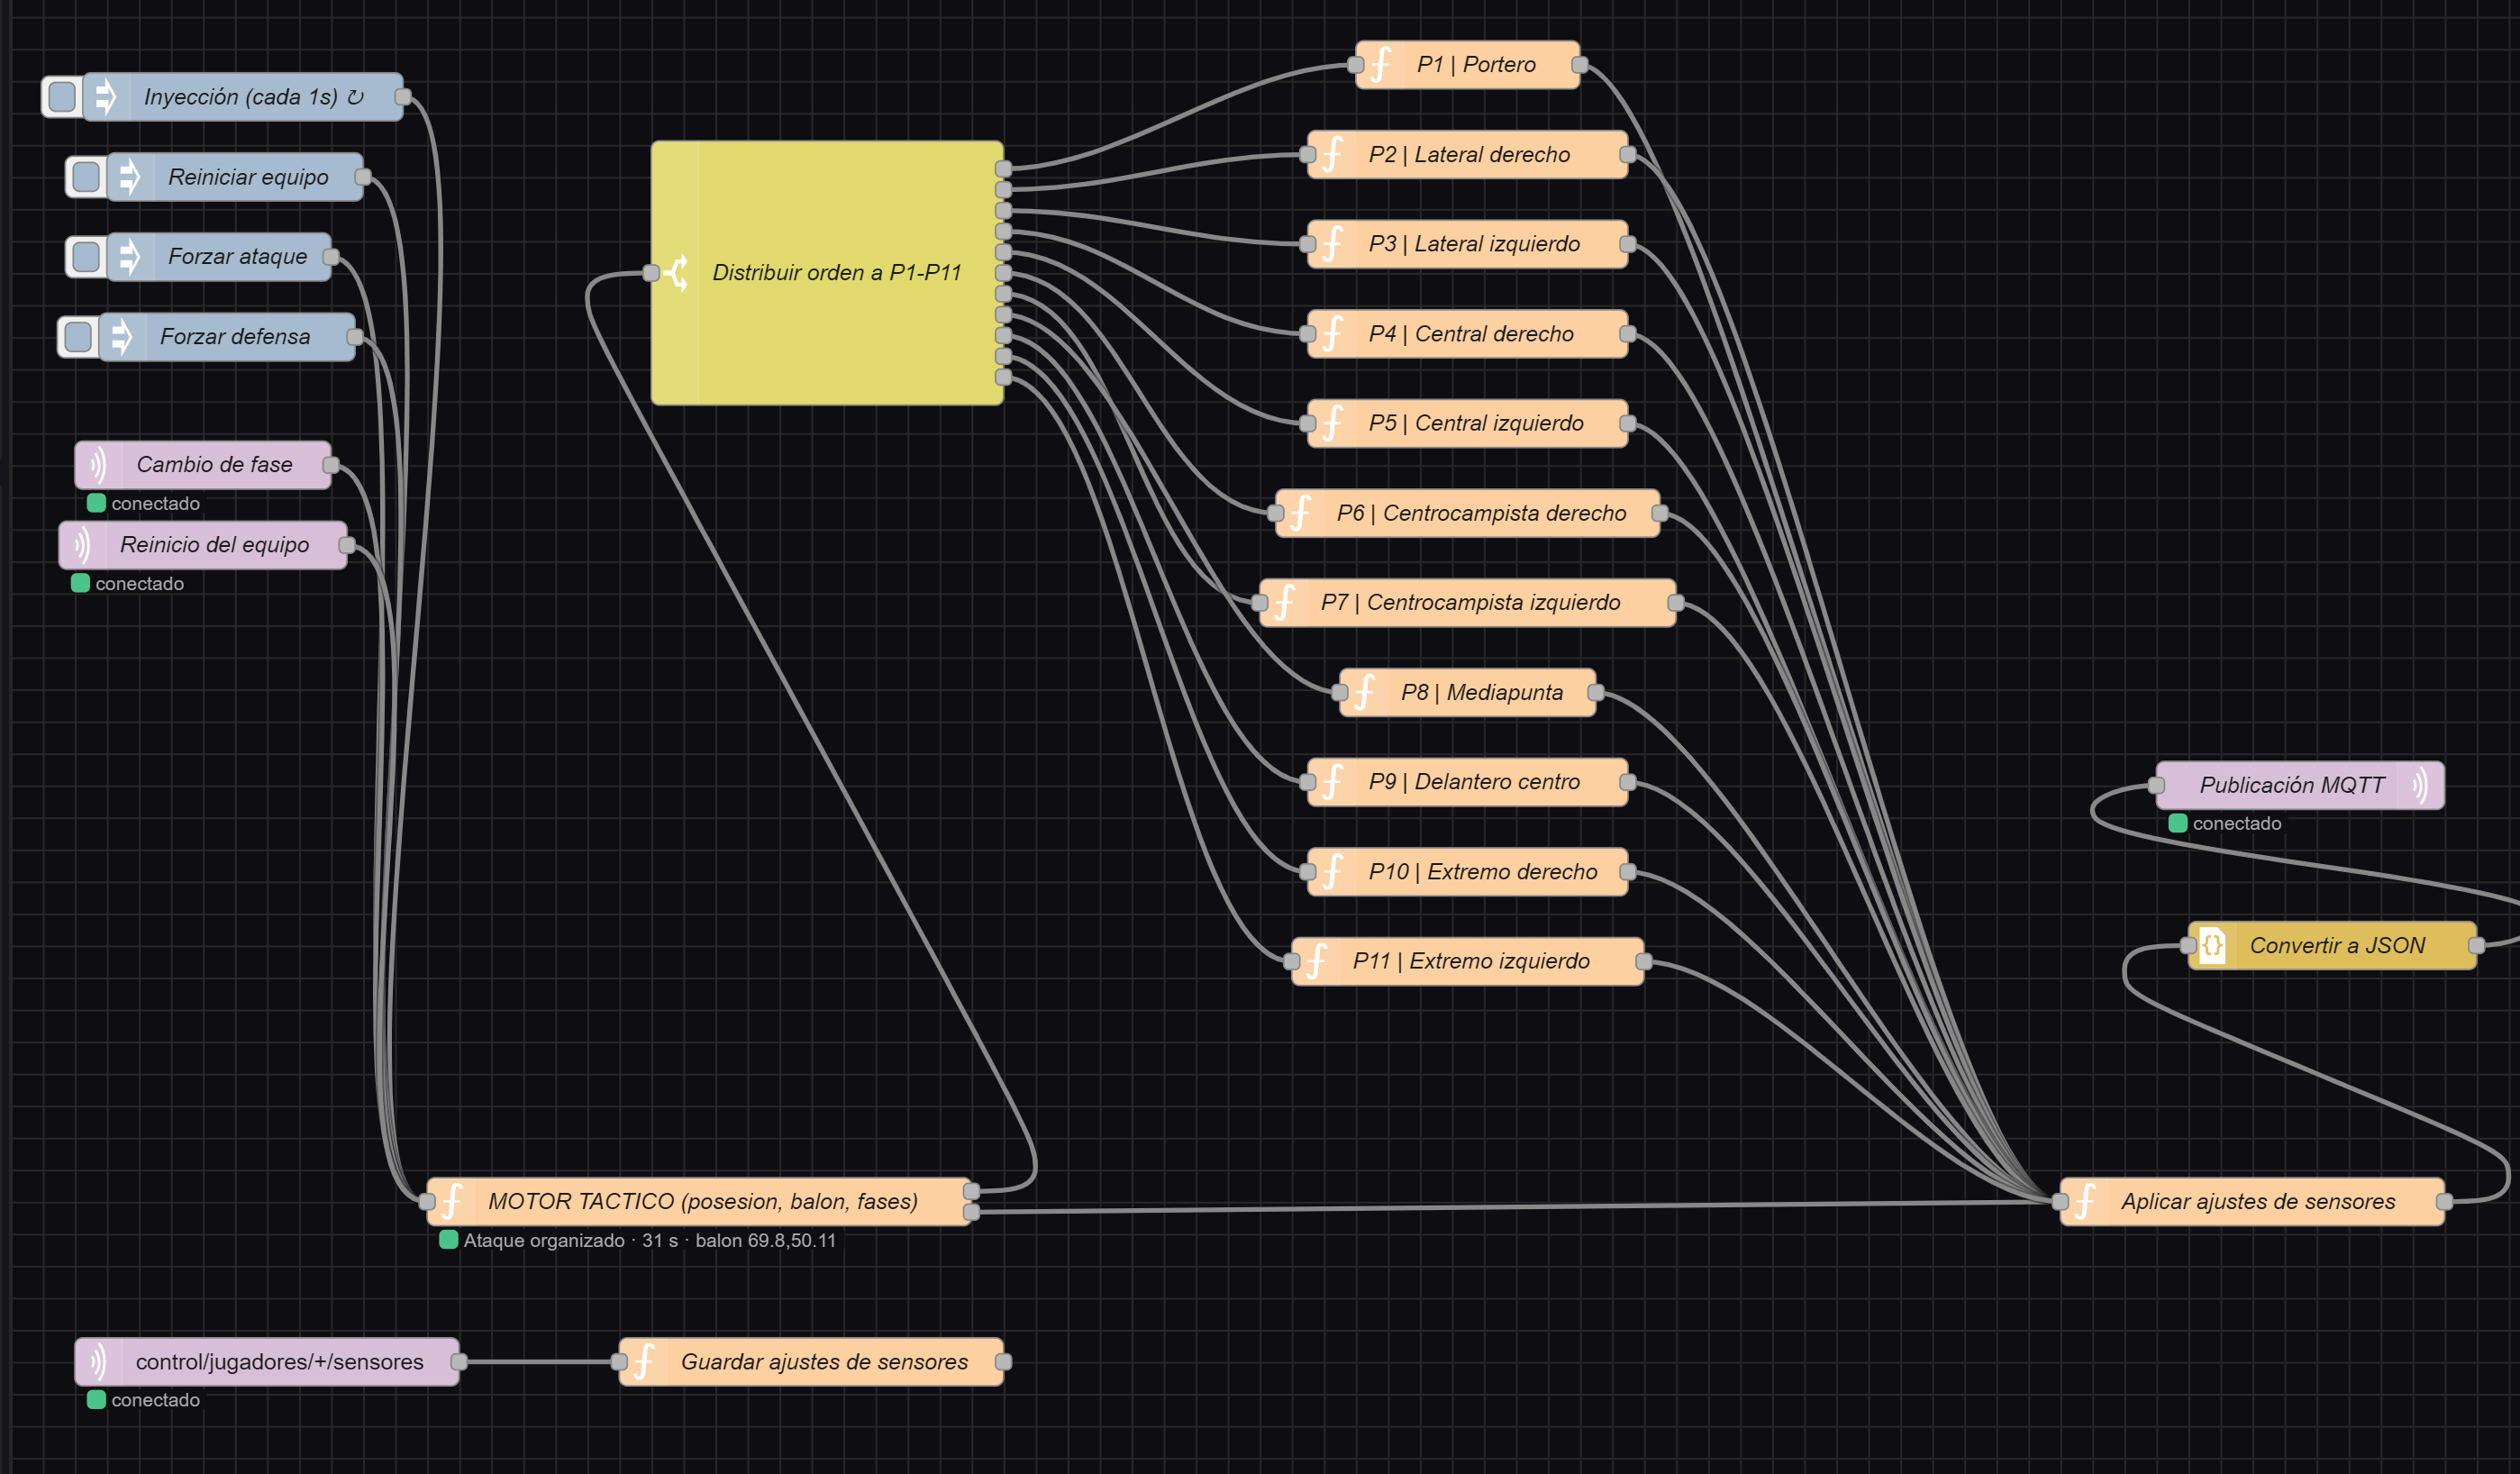
\includegraphics[width=\textwidth]{nr-simulador.png}
\caption{Flujo del simulador. El \texttt{inject} de cada segundo dispara el motor táctico; el \texttt{switch} reparte una orden a cada uno de los 11 \texttt{function} de jugador; \emph{Aplicar ajustes de sensores} sustituye los valores forzados; el nodo \texttt{json} serializa y \texttt{mqtt out} publica. Abajo, los \texttt{mqtt in} de \topic{control/\#}.}
\label{fig:nr-simulador}
\end{figure}

\begin{table}[!htbp]
\centering
\caption{Nodos del flujo del simulador.}\label{tab:nodos-sim}
\footnotesize
\begin{tabularx}{\textwidth}{p{2.4cm}p{0.6cm}L}
\toprule
\textbf{Nodo} & \textbf{Nº} & \textbf{Función} \\
\midrule
\texttt{inject} & 4 & Reloj de 1~s, reiniciar equipo, forzar ataque y forzar defensa \\
\texttt{mqtt in} & 3 & \topic{control/fase}, \topic{control/reset} y \topic{control/jugadores/+/sensores} (QoS 1) \\
\texttt{function} & 14 & Motor táctico, 11 jugadores, guardar y aplicar ajustes de sensores \\
\texttt{switch} & 1 & Reparte las órdenes según \texttt{msg.player} (11 salidas) \\
\texttt{json} & 1 & Convierte cada payload a texto JSON \\
\texttt{mqtt out} & 1 & Publica en el topic de cada mensaje (QoS 0) \\
\bottomrule
\end{tabularx}
\end{table}

\subsection{Flujo \emph{Pasarela MQTT $\rightarrow$ API}}

La pasarela (Fig.~\ref{fig:nr-pasarela}) se suscribe a \topic{+/sensors/\#} y guarda cada sensor en su jugador (contexto del flujo). Cada segundo, \emph{Montar lote} construye un único \texttt{POST /api/telemetria} con la última lectura de cada jugador y hace de \emph{watchdog}: si un jugador lleva 5~s sin datos, lo envía con \texttt{estado: "sin\_senal"}. La respuesta de la API (\texttt{202 · 11 recibidas}) se ve en el estado del nodo. Una segunda rama reenvía \topic{equipo/estado} a \texttt{POST /api/equipo/estado} para dibujar el balón y la fase en el campograma.

\begin{figure}[!htbp]
\centering
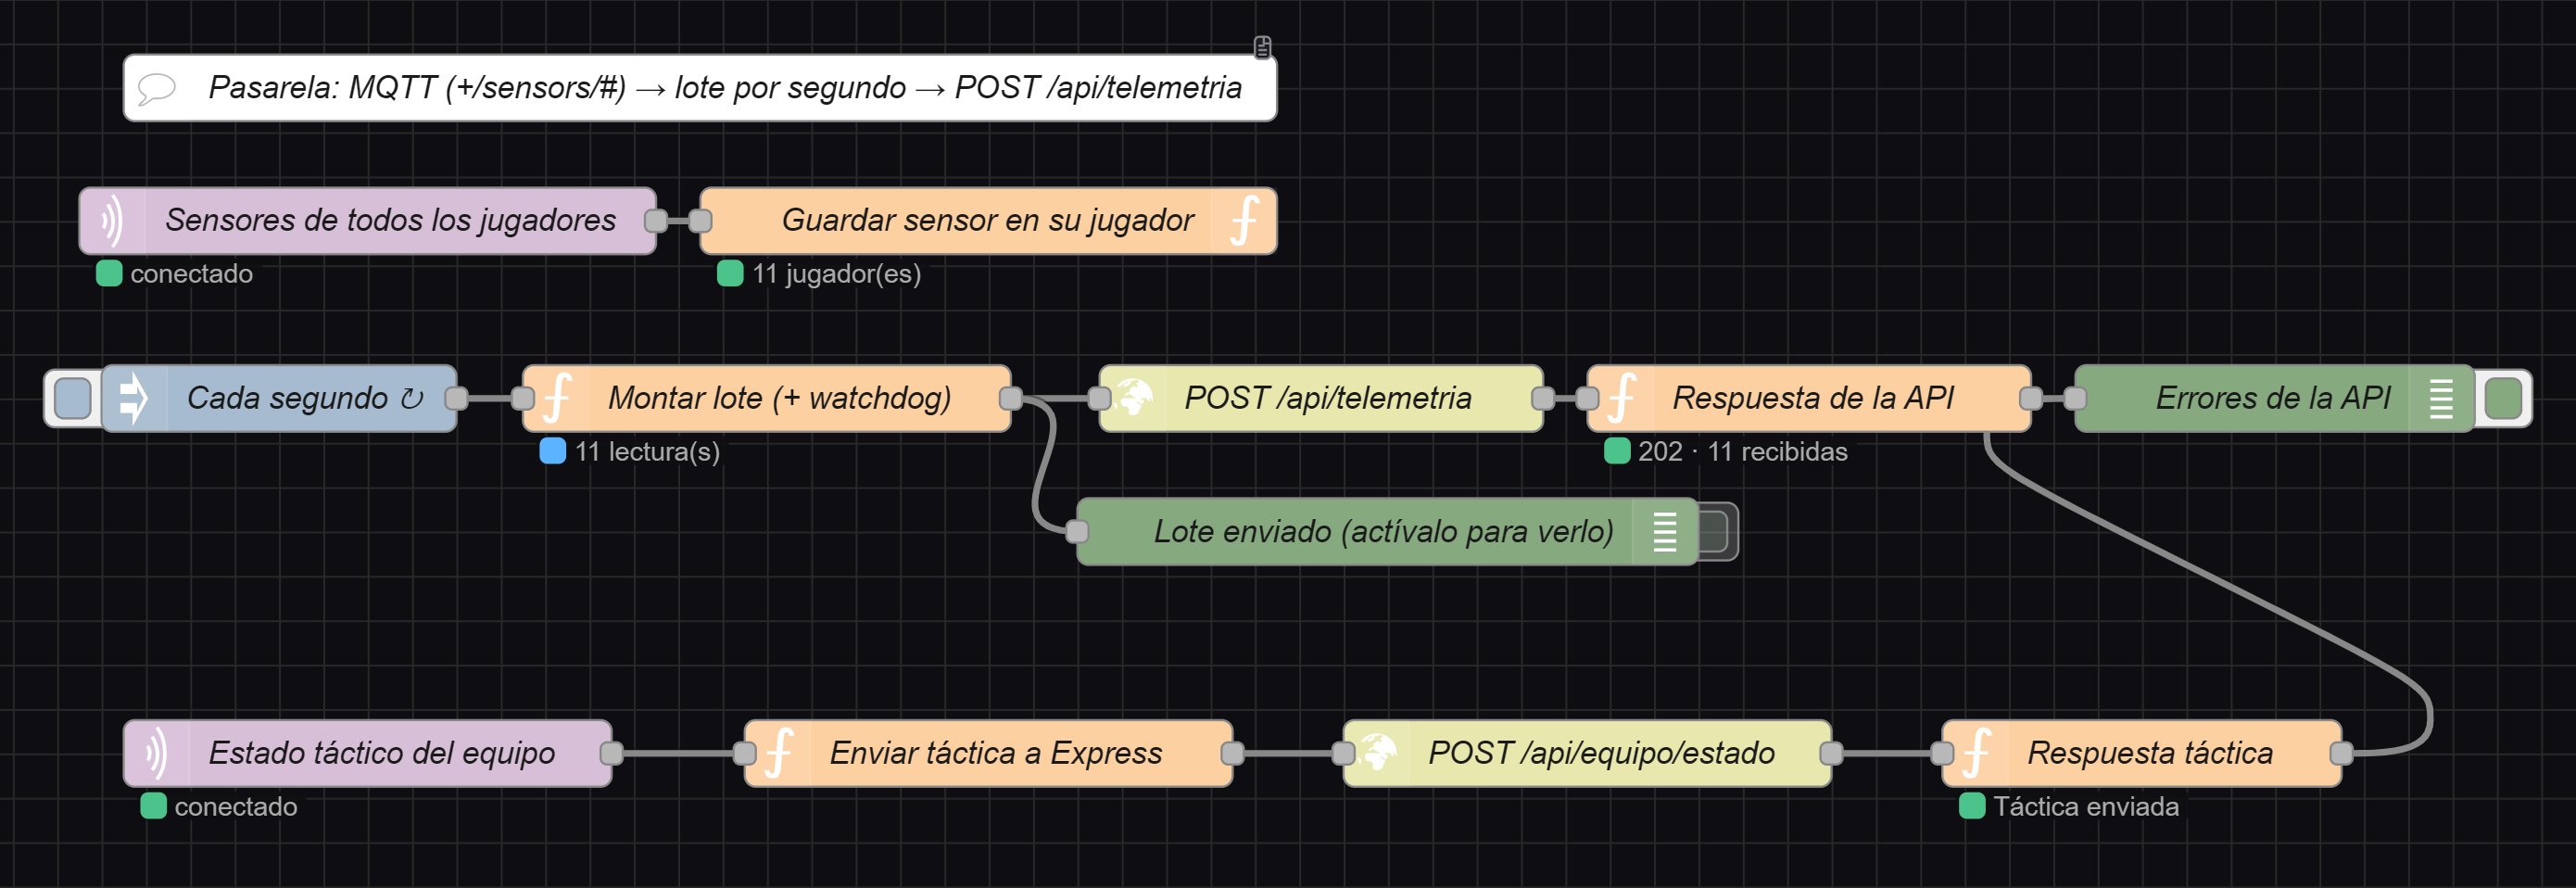
\includegraphics[width=\textwidth]{nr-pasarela.png}
\caption{Flujo de la pasarela: \texttt{mqtt in} $\rightarrow$ guardar sensor $\rightarrow$ lote por segundo con \emph{watchdog} $\rightarrow$ \texttt{http request} (POST) $\rightarrow$ respuesta de la API.}
\label{fig:nr-pasarela}
\end{figure}

En total los dos flujos usan los nodos \texttt{inject}, \texttt{function}, \texttt{switch}, \texttt{json}, \texttt{mqtt in}, \texttt{mqtt out}, \texttt{http request}, \texttt{debug} y \texttt{comment}.

%%%%%%%%%%%%%%%%%%%%%%%%%%%%%%%%%%%%%%%%%%%%%%%%%%%%%%%%%%%%%%%%%%%%%%%%%%%%%%
\section{API REST y cómo invocarla}\label{sec:api}
%%%%%%%%%%%%%%%%%%%%%%%%%%%%%%%%%%%%%%%%%%%%%%%%%%%%%%%%%%%%%%%%%%%%%%%%%%%%%%

La API está hecha con Node.js 24 y Express 5 (carpeta \ruta{api/}) y sigue la estructura de los ejemplos de clase: \ruta{server.js} arranca el servidor HTTP y le ata el servidor WebSocket; \ruta{servers/http-server.js} monta los \emph{routers}; la lógica está en \ruta{services/} y los modelos de MongoDB en \ruta{models/} (Fig.~\ref{fig:api-mod}).

\begin{itemize}
  \item \textbf{URL base:} \url{http://localhost:3000}. Peticiones y respuestas en JSON; fechas en ISO 8601 (UTC).
  \item \textbf{Documentación interactiva:} Swagger UI en \url{http://localhost:3000/api-docs}, generada desde \ruta{api/openapi.yaml} (OpenAPI 3.0.3, 21 rutas).
  \item \textbf{Contrato completo:} \ruta{docs/contratos/api.md}.
\end{itemize}


\begin{figure}[!htbp]
\centering
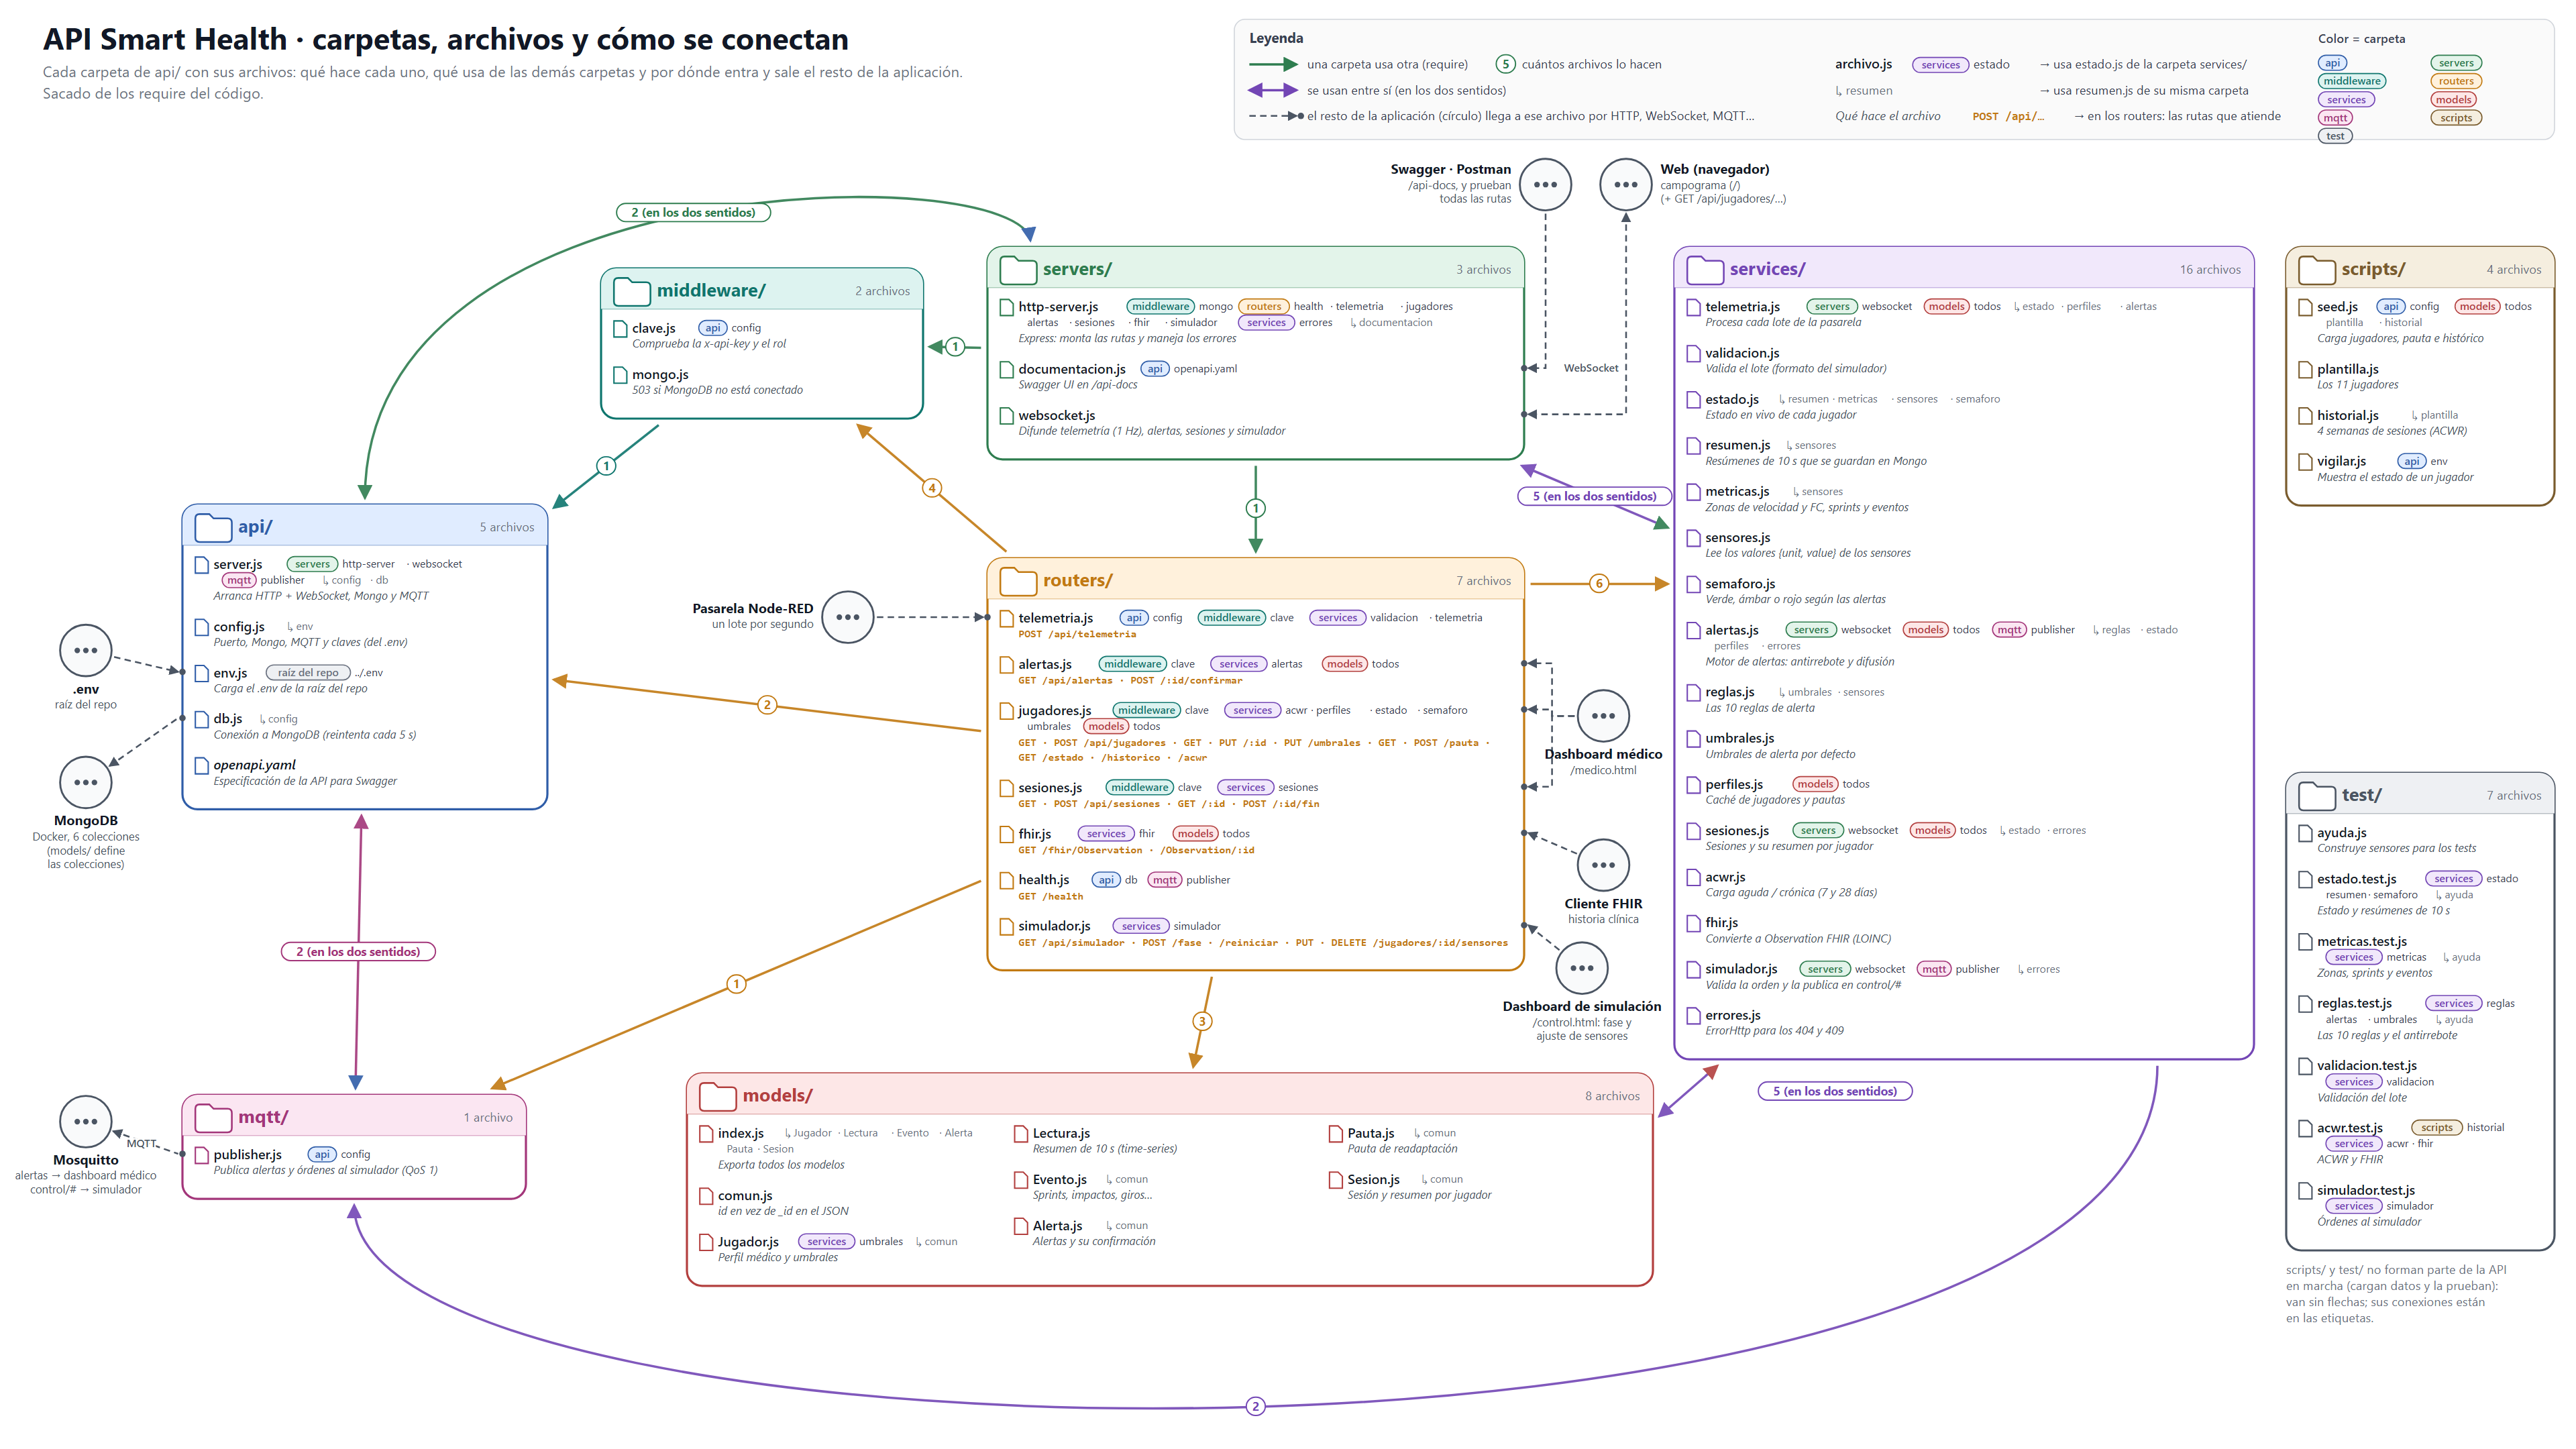
\includegraphics[width=\textwidth]{api-modulos.png}
\caption{Carpetas y archivos de la API, qué hace cada uno y quién entra por dónde.}
\label{fig:api-mod}
\end{figure}

\subsection{Operaciones}

Las operaciones de lectura no piden clave. Las que escriben datos clínicos piden la cabecera \texttt{x-api-key} con el rol adecuado (\emph{pasarela} o \emph{médico}).

\begin{table}[!htbp]
\centering
\caption{Operaciones de la API.}\label{tab:operaciones}
\scriptsize
\begin{tabularx}{\textwidth}{>{\raggedright\arraybackslash}p{1.1cm}>{\raggedright\arraybackslash}p{4.6cm}>{\raggedright\arraybackslash}p{1.15cm}L}
\toprule
\textbf{Método} & \textbf{Ruta} & \textbf{Clave} & \textbf{Para qué} \\
\midrule
POST & \ruta{/api/telemetria} & pasarela & Lote por segundo con la última lectura de cada jugador \\
GET\newline POST & \ruta{/api/equipo/estado} & —\newline pasarela & Estado táctico (balón, fase) para el campograma \\
GET\newline POST & \ruta{/api/jugadores} & —\newline médico & Lista de jugadores · alta de uno nuevo \\
GET\newline PUT & \ruta{/api/jugadores/:id} & —\newline médico & Perfil médico (FCmáx, temperatura basal, asimetría base\ldots) \\
PUT & \ruta{/api/jugadores/:id/umbrales} & médico & Ajustar los umbrales de alerta de un jugador \\
GET & \ruta{/api/jugadores/:id/estado} & — & Estado en vivo, valores derivados y semáforo \\
GET & \ruta{/api/jugadores/:id/historico} & — & Resúmenes de 10~s entre dos fechas (\texttt{?desde=\&hasta=}) \\
GET & \ruta{/api/jugadores/:id/acwr} & — & Ratio de carga aguda/crónica \\
GET\newline POST & \ruta{/api/jugadores/:id/pauta} & —\newline médico & Pauta de readaptación activa · crear una nueva \\
GET & \ruta{/api/alertas} & — & Alertas (\texttt{?estado=\&jugadorId=}) \\
POST & \ruta{/api/alertas/:id/confirmar} & médico & El médico confirma una alerta \\
GET\newline POST & \ruta{/api/sesiones} & —\newline médico & Lista de sesiones · empezar una \\
GET & \ruta{/api/sesiones/:id} & — & Una sesión con su resumen por jugador \\
POST & \ruta{/api/sesiones/:id/fin} & médico & Cerrar la sesión y guardar el resumen \\
GET & \ruta{/api/simulador} & — & Fases válidas, rangos y última orden enviada \\
POST & \ruta{/api/simulador/fase}, \ruta{/reiniciar} & — & Cambiar la fase de juego o reiniciar el simulador \\
PUT\newline DELETE & \ruta{/api/simulador/jugadores/:id/sensores} & — & Forzar (o dejar de forzar) el pulso o la temperatura \\
GET & \ruta{/fhir/Observation} & — & Constantes vitales en FHIR R4 (\texttt{?patient=\&code=}) \\
GET & \ruta{/fhir/Observation/:id} & — & Una \texttt{Observation} \\
GET & \ruta{/health} & — & Estado de la API, de MongoDB y del broker \\
\bottomrule
\end{tabularx}
\end{table}

\textbf{Errores.} Todas las rutas responden \texttt{\{"error": "mensaje"\}} con su código: \texttt{400} (cuerpo o parámetros no válidos, indicando el campo), \texttt{401} (falta la clave o no es válida), \texttt{403} (la clave no tiene ese rol), \texttt{404}, \texttt{409} (ya existe, ya está confirmada o ya hay una sesión abierta) y \texttt{503} (MongoDB o Mosquitto no disponibles). Las rutas FHIR devuelven los errores como \texttt{OperationOutcome}.

\subsection{El lote de telemetría}

La pasarela envía cada segundo un lote con la última lectura de cada jugador. \textbf{La API no traduce nada}: cada bloque de \texttt{sensors} es exactamente el payload que el simulador publica por MQTT.

\begin{lstlisting}[language=json]
POST /api/telemetria        x-api-key: <API_KEY_PASARELA>
{ "ts": "2026-11-12T18:30:05.000Z",
  "lecturas": [
    { "jugadorId": "p8", "estado": "ok", "sensors": {
        "gps": { "speed": {"unit":"km/h","value":28.7}, "distancecovered": {"unit":"m","value":7842},
                 "position": {"X":{"unit":"m","value":52.3}, "Y":{"unit":"m","value":30.1}} },
        "pulsemeter": { "pulse": {"unit":"bpm","value":181} }, ... } },
    { "jugadorId": "p10", "estado": "sin_senal" } ] }
→ 202 Accepted   {"recibidas": 11, "ignoradas": []}
\end{lstlisting}

La validación (\ruta{services/validacion.js}) comprueba el tipo, la unidad y el rango de cada medida (una velocidad en m/s en vez de km/h se rechaza). Si algo falla, rechaza el lote entero indicando la lectura y el campo, por ejemplo \texttt{lecturas[3]: sensors.pulsemeter.pulse.value debe ser un número}.

\subsection{Cómo invocarla}

\textbf{Desde Swagger UI.} En \url{http://localhost:3000/api-docs}, el botón \emph{Authorize} pide la \texttt{x-api-key} y cada operación se puede probar con \emph{Try it out $\rightarrow$ Execute} (Figs.~\ref{fig:swagger} y~\ref{fig:swagger-sim}).

\begin{figure}[!htbp]
\centering
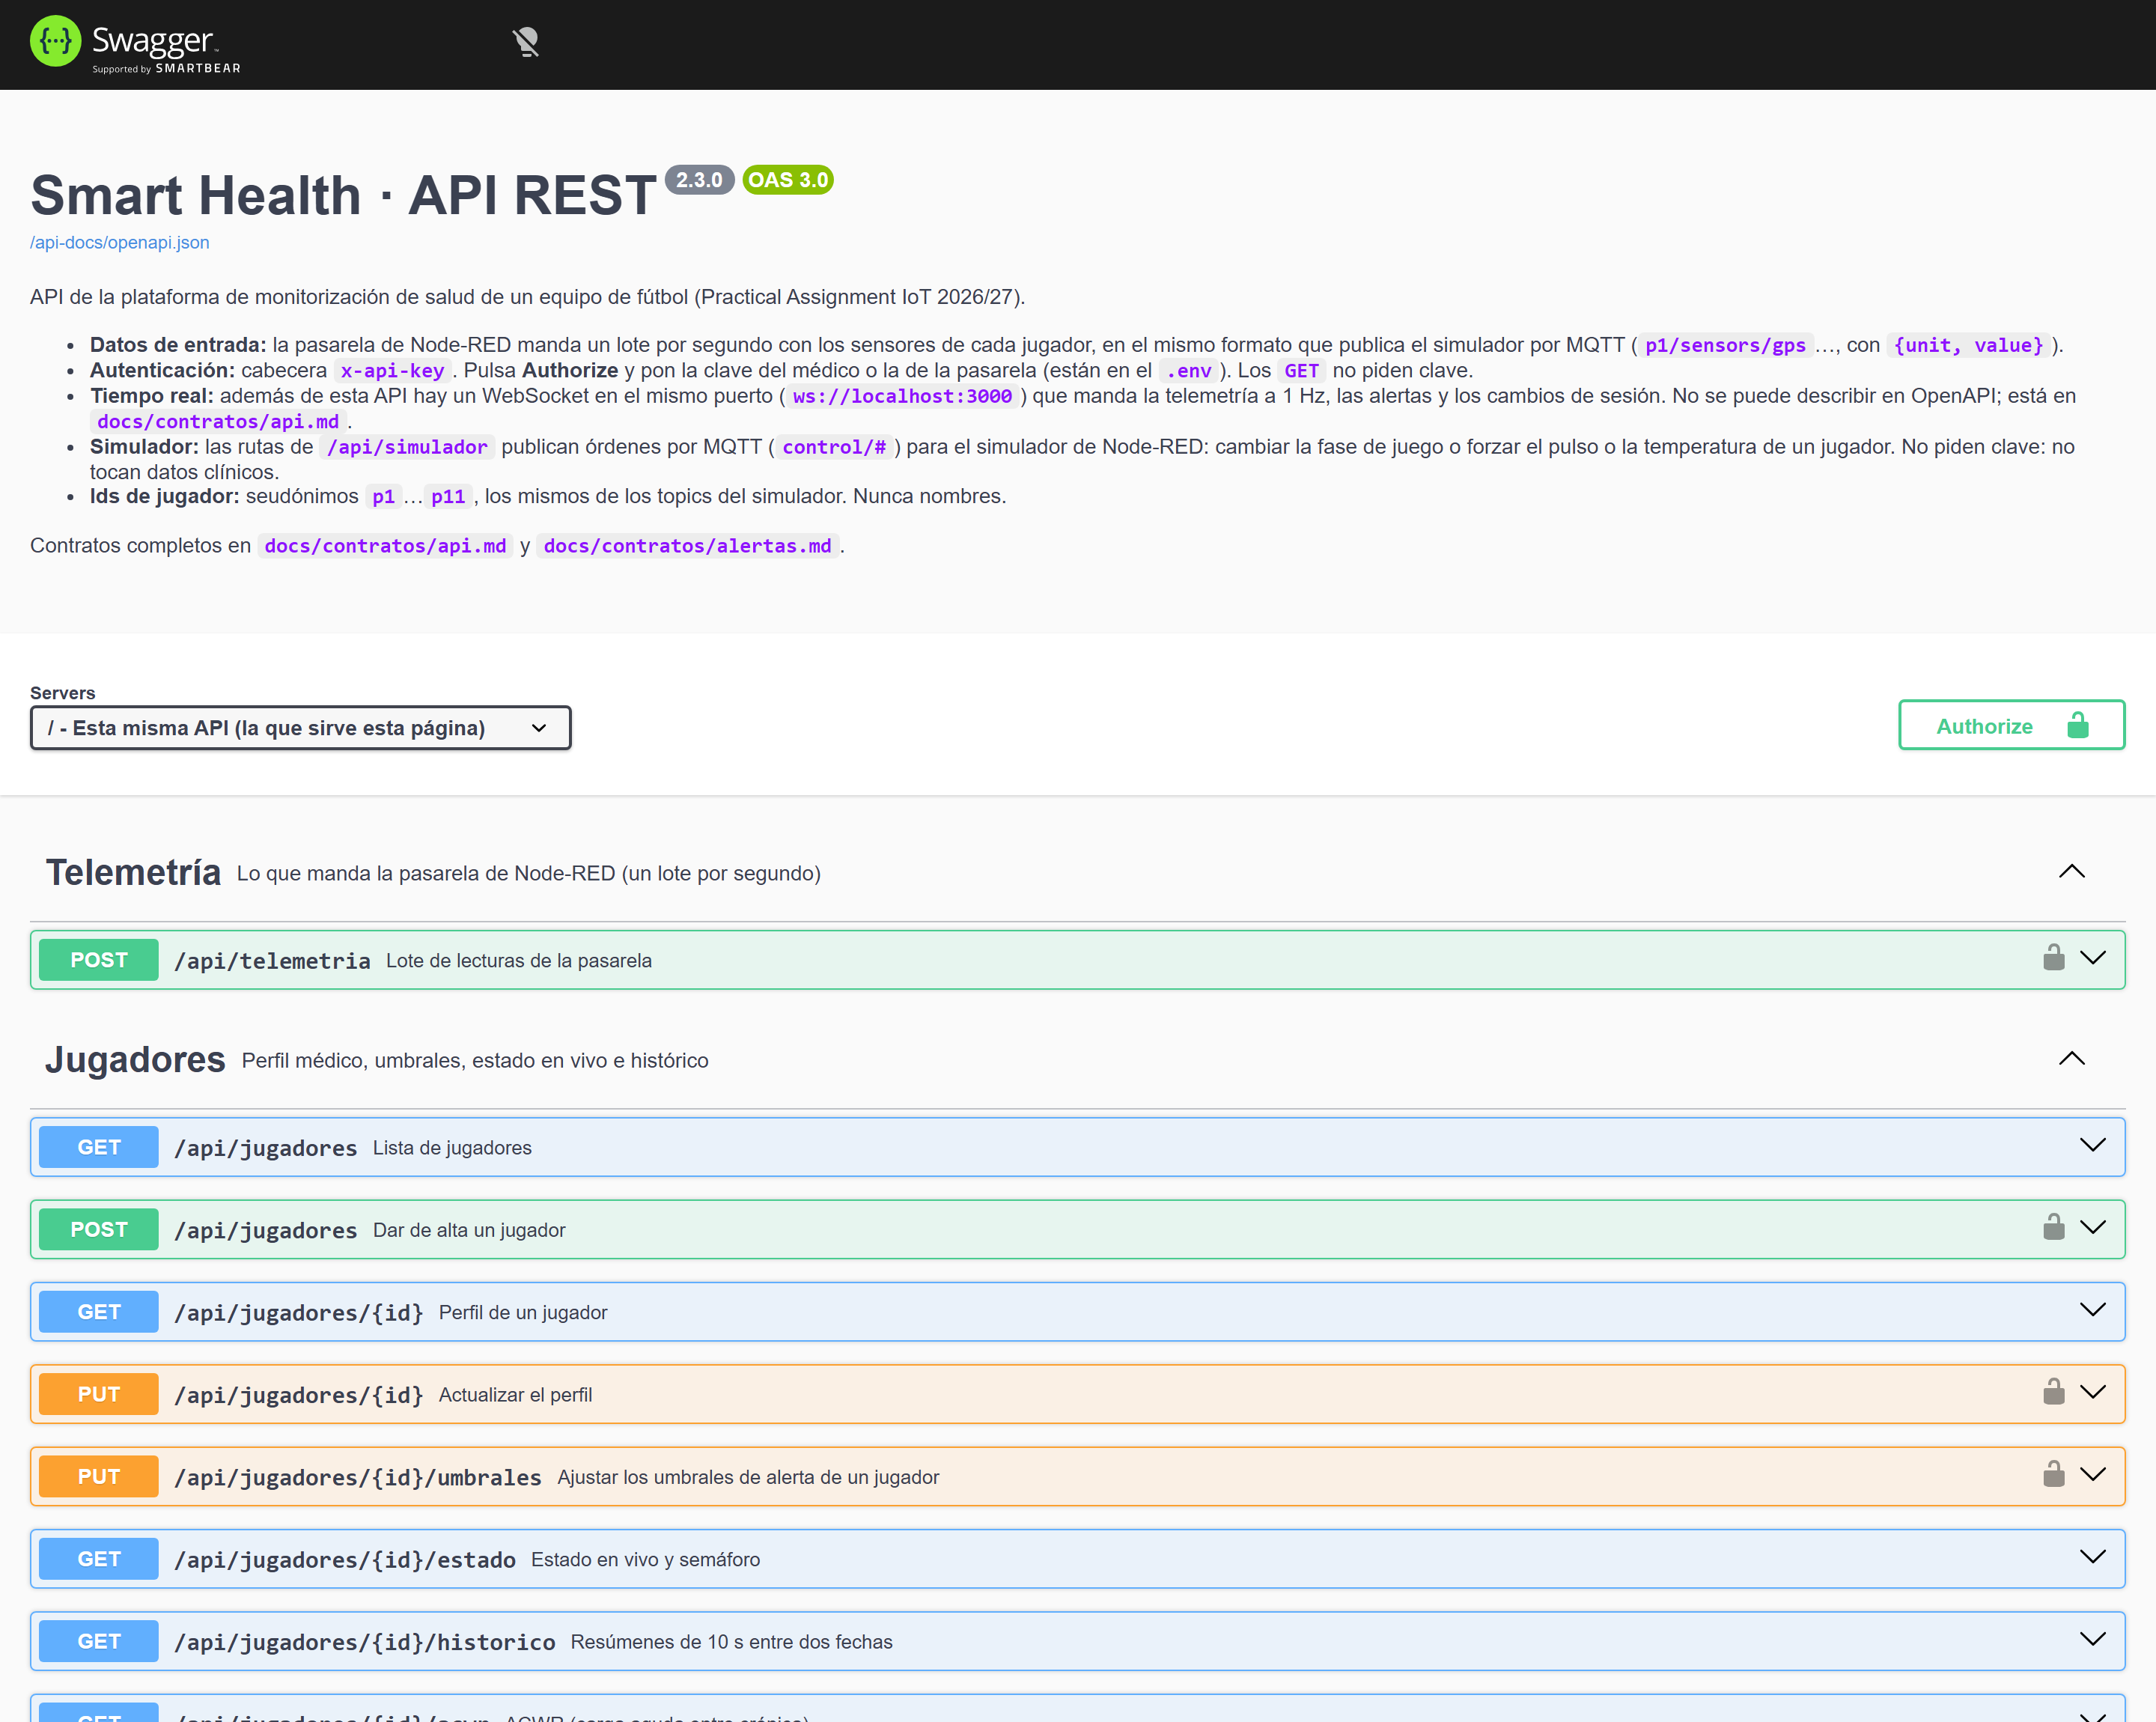
\includegraphics[width=0.8\textwidth]{swagger.png}
\caption{Swagger UI con las operaciones de la API agrupadas por recurso.}
\label{fig:swagger}
\end{figure}

\begin{figure}[!htbp]
\centering
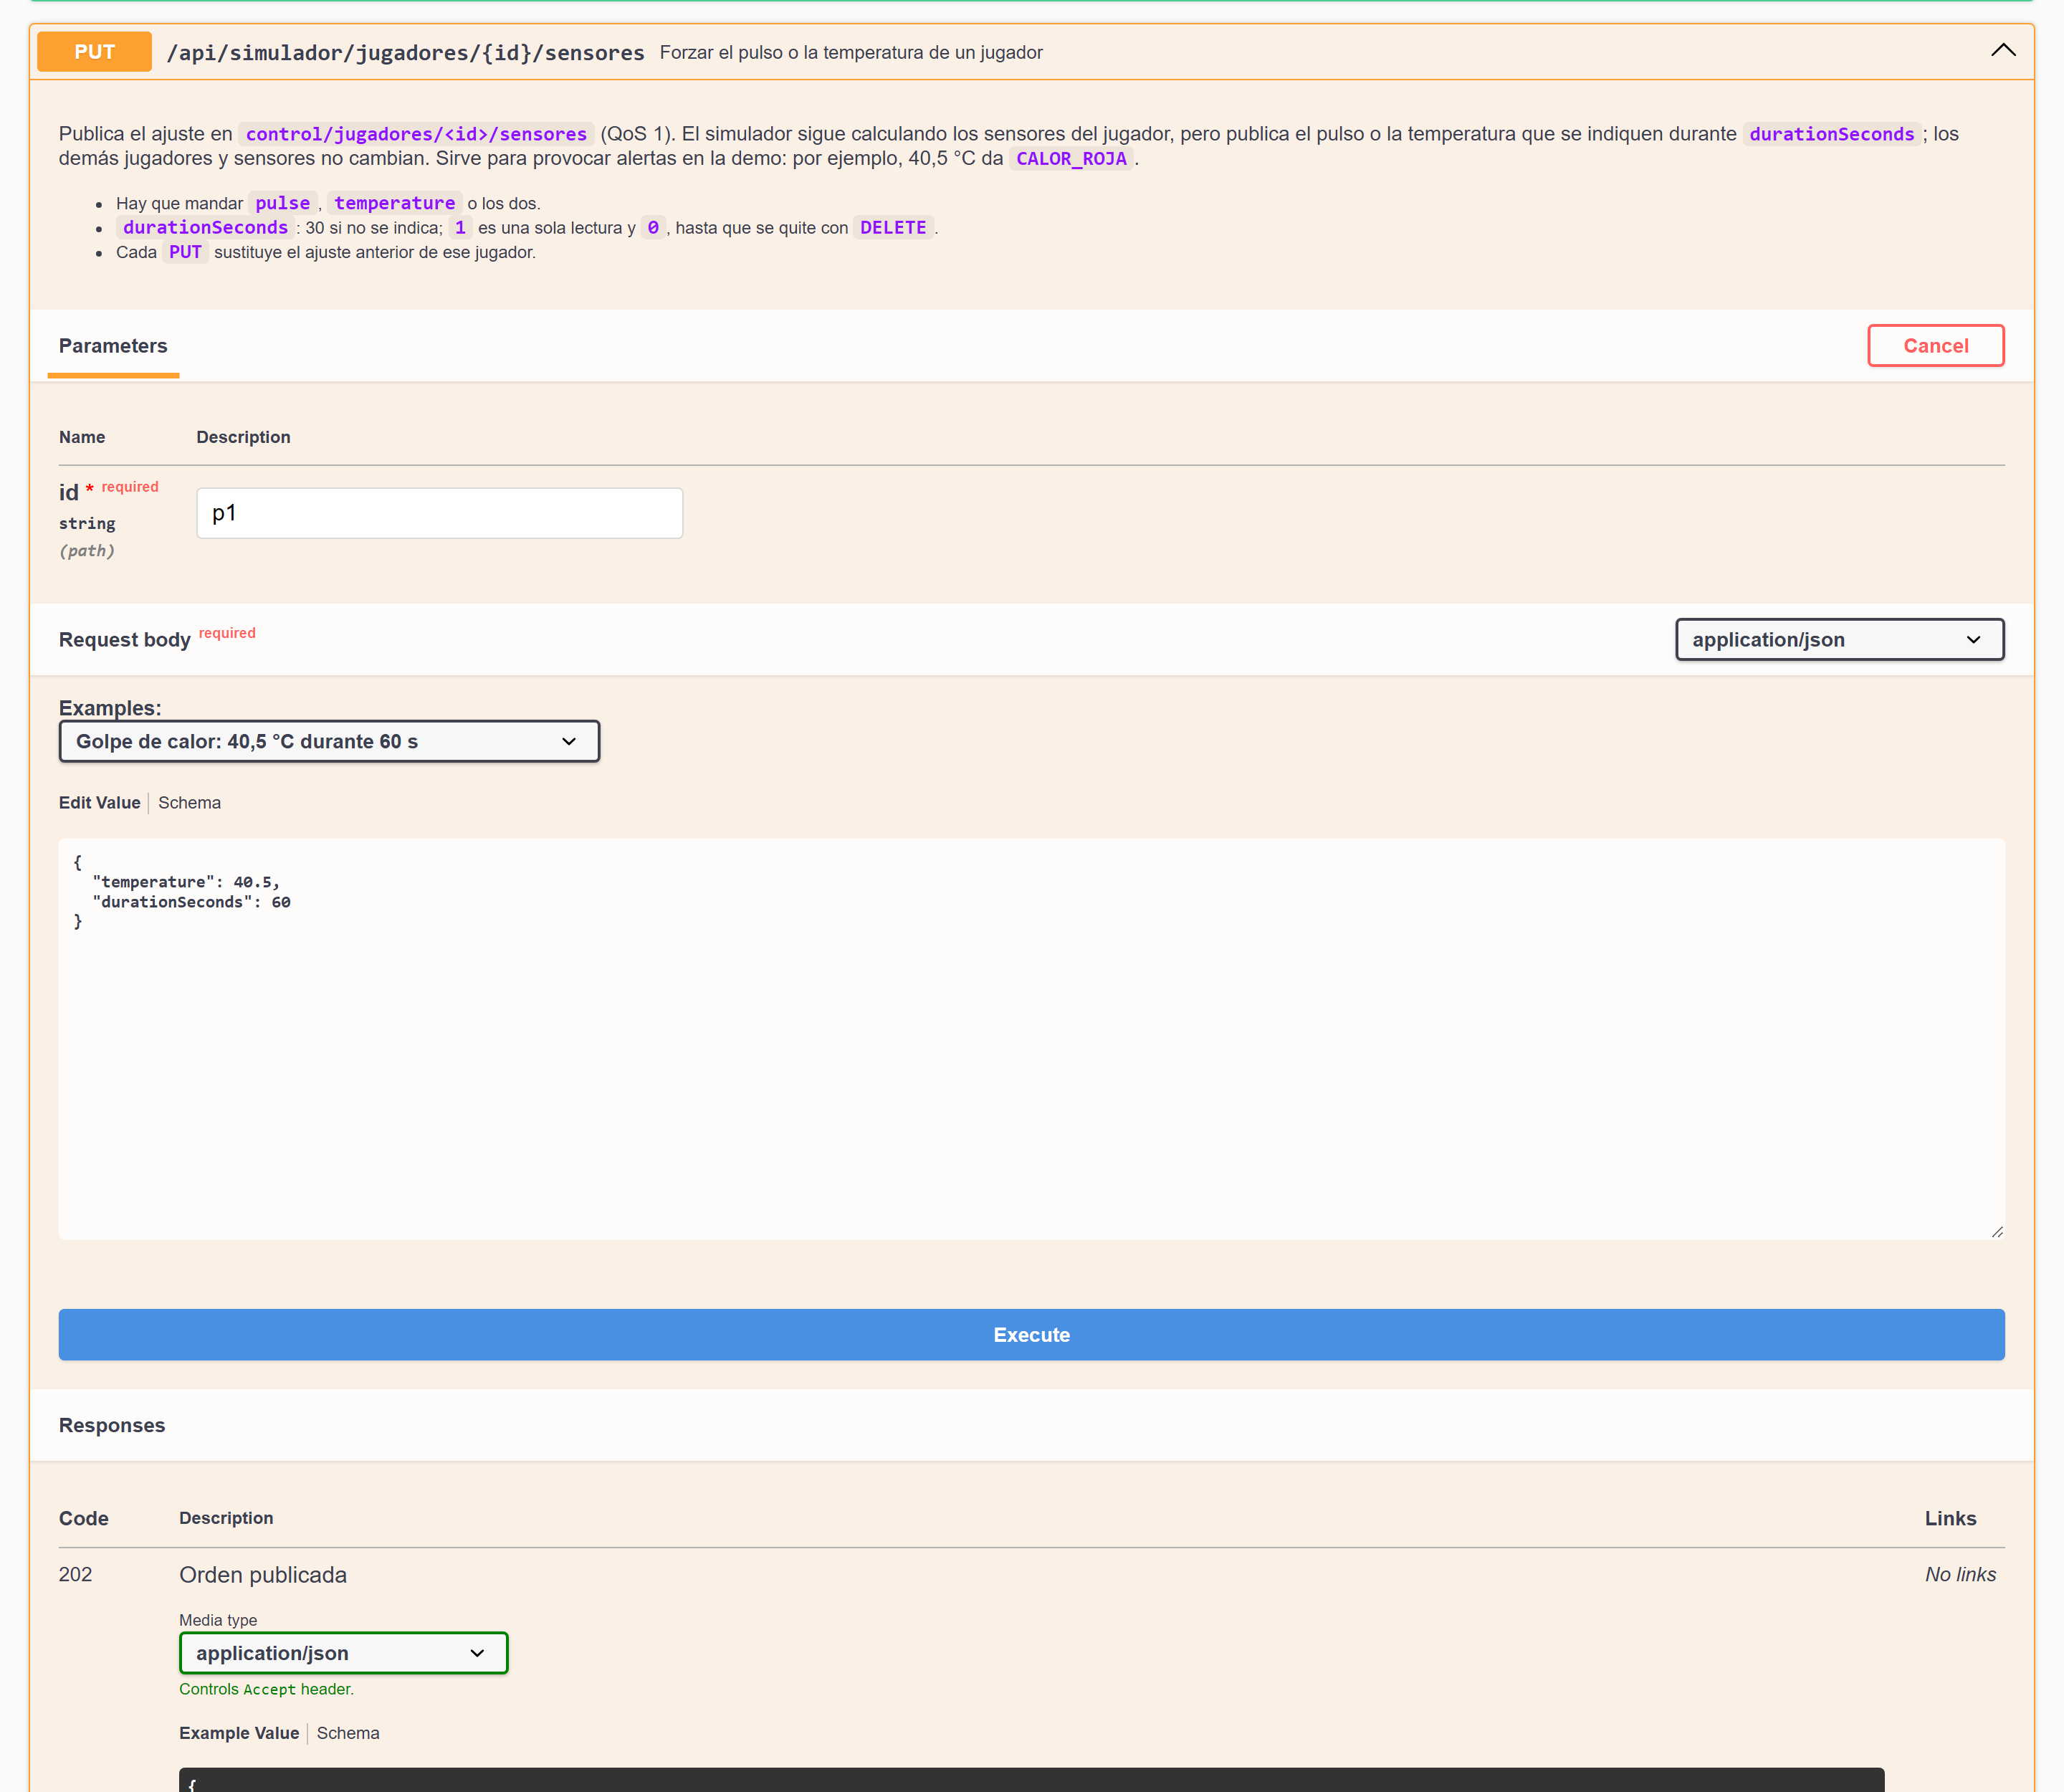
\includegraphics[width=0.8\textwidth]{swagger-simulador.png}
\caption{La operación para forzar un valor del simulador en Swagger, con sus ejemplos.}
\label{fig:swagger-sim}
\end{figure}

\textbf{Desde Postman.} El fichero \ruta{docs/postman\_collection.json} tiene 47 peticiones en 11 carpetas (una por recurso más una de errores). Las claves se ponen en el \emph{Current value} de las variables \texttt{claveMedico} y \texttt{clavePasarela}, así que no se guardan en el fichero. Las peticiones encadenan datos entre sí (al empezar una sesión se guarda su id para cerrarla después) y cada una comprueba su código de respuesta, de modo que la colección entera se puede lanzar con el \emph{Collection Runner}.

\textbf{Con curl} (en PowerShell, \texttt{curl.exe}):

\begin{lstlisting}[language=shell]
# Estado en vivo de un jugador (no pide clave)
curl http://localhost:3000/api/jugadores/p8/estado

# El médico confirma una alerta
curl -X POST http://localhost:3000/api/alertas/6733f0c2a1b2c3d4e5f60718/confirmar \
     -H "Content-Type: application/json" -H "x-api-key: <API_KEY_MEDICO>" \
     -d '{"por": "Dra. Pérez", "nota": "Retirado a la banda, hidratación"}'

# Golpe de calor a p8 durante 60 s
curl -X PUT http://localhost:3000/api/simulador/jugadores/p8/sensores \
     -H "Content-Type: application/json" -d '{"temperature": 40.5, "durationSeconds": 60}'

# Frecuencia cardiaca en FHIR
curl "http://localhost:3000/fhir/Observation?patient=p8&code=8867-4&_count=5"
\end{lstlisting}

\textbf{Desde un cliente web}, con \texttt{fetch} para REST y \texttt{WebSocket} para el tiempo real, que es lo que hace el campograma:

\begin{lstlisting}[language=js]
const estado = await fetch('http://localhost:3000/api/jugadores/p8/estado').then(r => r.json());

const ws = new WebSocket('ws://localhost:3000');
ws.onmessage = function (e) {
    const msg = JSON.parse(e.data);
    if (msg.tipo === 'telemetria') pintarCampo(msg.jugadores);   // 1 Hz
    if (msg.tipo === 'alerta') avisar(msg.alerta);                // al momento
};
\end{lstlisting}

\subsection{Las rutas del simulador}

Las rutas de \ruta{/api/simulador} responden \texttt{202 Accepted}: la API no espera a que el simulador cambie, solo a que el broker confirme la publicación (PUBACK). Devuelven \texttt{400} con la lista de fases válidas o el rango permitido, \texttt{404} si el jugador no es de \texttt{p1} a \texttt{p11}, \texttt{503} si la API no está conectada a Mosquitto y \texttt{502} si el broker no confirma. No piden clave ni MongoDB porque no tocan datos clínicos; en producción no existirían.

%%%%%%%%%%%%%%%%%%%%%%%%%%%%%%%%%%%%%%%%%%%%%%%%%%%%%%%%%%%%%%%%%%%%%%%%%%%%%%
\section{Motor de alertas}
%%%%%%%%%%%%%%%%%%%%%%%%%%%%%%%%%%%%%%%%%%%%%%%%%%%%%%%%%%%%%%%%%%%%%%%%%%%%%%

\subsection{Funcionamiento}

Cada segundo, por cada jugador del lote:

\begin{enumerate}
  \item \textbf{Estado en vivo} (\ruta{services/estado.js}). Se guardan en memoria sus últimos sensores, un historial de 180~s y unos valores derivados: \% de la FC máxima, zona de FC (Z1--Z5), zona de velocidad (andar, trote, carrera, alta intensidad y \emph{sprint}) y asimetría de carga entre pies. También se acumulan los datos de la sesión: distancia, metros a alta intensidad ($>19{,}8$~km/h), \emph{sprints} ($>25$~km/h) y acciones de alta intensidad ($>3$~m/s$^2$).
  \item \textbf{Reglas} (\ruta{services/reglas.js}). Diez funciones puras que reciben el estado del jugador, su perfil (con sus umbrales) y su pauta, y devuelven la alerta o nada.
  \item \textbf{Antirrebote} (\ruta{services/alertas.js}). Una alerta no se repite para el mismo jugador mientras siga activa, ni durante los 60~s siguientes a que el médico la confirme.
  \item \textbf{Difusión.} Cada alerta nueva se guarda en MongoDB, se publica por MQTT en \topic{sensors/eq1/alertas} con QoS 1 y se envía por WebSocket.
\end{enumerate}

El \textbf{semáforo} de cada jugador sale de sus alertas activas: rojo si alguna es crítica, ámbar si hay algún aviso y verde si no hay ninguna. Las alertas no se cierran solas: siguen activas hasta que el médico las confirma.

\begin{lstlisting}[language=json]
{ "id": "6733f0c2a1b2c3d4e5f60718", "jugadorId": "p8", "codigo": "CALOR_ROJA",
  "severidad": "critica", "mensaje": "Temperatura interna de 40,5 °C (umbral 40 °C)",
  "valor": 40.5, "umbral": 40, "ts": "2026-11-16T22:58:01.229Z", "estado": "activa",
  "confirmadaPor": null, "confirmadaEn": null, "nota": null }
\end{lstlisting}

\subsection{Reglas y umbrales}

Los umbrales son valores por defecto; cada jugador guarda su propia copia, que el médico ajusta con \texttt{PUT /api/jugadores/:id/umbrales}.

\begin{table}[!htbp]
\centering
\caption{Reglas de alerta.}\label{tab:reglas}
\scriptsize
\begin{tabularx}{\textwidth}{p{2.8cm}Lp{2.1cm}p{1.1cm}}
\toprule
\textbf{Código} & \textbf{Se dispara cuando\ldots} & \textbf{Por defecto} & \textbf{Severidad} \\
\midrule
\texttt{CALOR\_AMBAR} & Temperatura interna $\geq$ \texttt{tempAmbar} & 39~$^\circ$C & aviso \\
\texttt{CALOR\_ROJA} & Temperatura interna $\geq$ \texttt{tempRoja} & 40~$^\circ$C & crítica \\
\texttt{FC\_ALTA} & FC por encima del \texttt{fcAltaPct}~\% de la FCmáx durante \texttt{fcAltaSeg} & 92~\% · 60~s & aviso \\
\texttt{FC\_DESACOPLE} & FC $>85$~\% de la FCmáx caminando ($<7$~km/h) durante 30~s & 85~\% · 7~km/h · 30~s & aviso \\
\texttt{RECUPERACION\_LENTA} & Tras un esfuerzo (de $>19{,}8$ a $<7$~km/h), la FC baja 12~lpm o menos en 60~s & 12~lpm & aviso \\
\texttt{INCIDENTE} & Impacto $\geq4$~g, inmóvil 10~s y luego FC anómala ($<50$~lpm o $>95$~\% FCmáx) o sin señal & 4~g · 10~s & crítica \\
\texttt{SOBRECARGA} & Aceleraciones + desaceleraciones $>3$~m/s$^2$ en la sesión por encima del límite & 120 & aviso \\
\texttt{ASIMETRIA} & $|$media de (izq $-$ der) en 60~s$|$ supera la asimetría base en más del umbral (con al menos 45~s de datos) & 15 puntos & aviso \\
\texttt{PAUTA\_EXCEDIDA} & Con pauta activa: velocidad $>$ \texttt{velMax}, metros a alta intensidad $>$ \texttt{cargaMax} o asimetría $>$ \texttt{asimetriaMax} & los fija el médico & aviso \\
\texttt{SIN\_SENAL} & El \emph{watchdog} de la pasarela lleva 5~s sin datos del jugador & 5~s & aviso \\
\bottomrule
\end{tabularx}
\end{table}

\subsection{Justificación de los umbrales}

\begin{itemize}
  \item \textbf{Calor.} En partidos con calor, el pico medio de temperatura interna de los futbolistas fue de 39,2~$^\circ$C (rango 37,9--40,1~$^\circ$C) \cite{tempfutbol,tempreview}. Por encima de 39~$^\circ$C empeora el \emph{sprint} repetido, y 40~$^\circ$C es el criterio clínico de golpe de calor.
  \item \textbf{Recuperación de la FC.} Una caída de 12~lpm o menos en el primer minuto tras el esfuerzo se asoció a mayor mortalidad en una cohorte clínica de 2.428 adultos \cite{cole1999}. Aquí es un indicador, no un diagnóstico.
  \item \textbf{Aceleraciones.} $\pm3$~m/s$^2$ mantenidos 0,5~s es el umbral habitual de alta intensidad \cite{statsports,scisports}. En partidos de academia de élite se han registrado hasta 46 aceleraciones y 73 desaceleraciones de alta intensidad; de ahí el límite de 120 por sesión.
  \item \textbf{Asimetría.} No hay un umbral validado \cite{plantillas}, por eso se compara con la línea base de cada jugador. Se usa la \textbf{media con signo} del último minuto: en cada pisada la carga pasa de un pie al otro y una lectura suelta puede marcar 20 o 30 puntos aunque el jugador esté bien; con la media esas alternancias se compensan y queda solo el desequilibrio mantenido.
  \item \textbf{ACWR.} Carga de los últimos 7 días entre la media semanal de 28 \cite{gabbett2016}: entre 0,8 y 1,3 se considera la ``zona óptima'' y por encima de 1,3 sube el riesgo. Es una referencia discutida \cite{impellizzeri2020}, así que se usa para vigilar picos de carga, no para predecir lesiones.
\end{itemize}

\subsection{Calibración con el simulador}

Al conectar el motor de alertas con el simulador de 11 jugadores, dos reglas saltaban en falso. Se ajustaron midiendo, no a ojo:

\begin{itemize}
  \item \texttt{SOBRECARGA} saltaba en todos los jugadores de campo a partir del minuto 33. El simulador limita la frenada a 3,0~m/s$^2$ justos y frena siempre a tope, así que con ``3 o más'' cada parada contaba como alta intensidad: de 2.811 frenadas altas, 2.787 eran exactamente 3,0. Ahora se cuentan las de \textbf{más} de 3~m/s$^2$.
  \item \texttt{ASIMETRIA} saltaba al arrancar (con una sola lectura, la ``media'' es una pisada) y, de vez en cuando, al moverse de lado (la media de un minuto llegó a 17,4 puntos en dos horas). Ahora hacen falta 45~s de datos y el umbral pasa de 10 a 15 puntos.
\end{itemize}

Tras los ajustes, en tres partidos simulados de dos horas con los once jugadores no saltó ninguna alerta falsa.

%%%%%%%%%%%%%%%%%%%%%%%%%%%%%%%%%%%%%%%%%%%%%%%%%%%%%%%%%%%%%%%%%%%%%%%%%%%%%%
\section{Base de datos, WebSockets y FHIR}
%%%%%%%%%%%%%%%%%%%%%%%%%%%%%%%%%%%%%%%%%%%%%%%%%%%%%%%%%%%%%%%%%%%%%%%%%%%%%%

\subsection{MongoDB}

MongoDB 8 se ejecuta en Docker (\ruta{docker-compose.yml}) y se accede con Mongoose.

\begin{table}[!htbp]
\centering
\caption{Colecciones de MongoDB.}\label{tab:colecciones}
\footnotesize
\begin{tabularx}{\textwidth}{p{1.8cm}Lp{3.1cm}}
\toprule
\textbf{Colección} & \textbf{Qué guarda} & \textbf{Notas} \\
\midrule
\texttt{jugadores} & Perfil médico con id seudónimo (\texttt{p1}\ldots\texttt{p11}), posición, FCmáx, temperatura basal, asimetría base y umbrales & Nunca nombres \\
\texttt{lecturas} & Resumen de 10~s por jugador: velocidad media y máxima, metros, metros a alta intensidad, FC media y máxima, temperatura, asimetría, \emph{sprints}, acciones altas y posición & Colección \emph{time-series} (\texttt{timeField: ts}, \texttt{metaField: jugadorId}) \\
\texttt{eventos} & \emph{Sprints}, aceleraciones y desaceleraciones altas, cambios de dirección e impactos & Para el informe del partido \\
\texttt{alertas} & Cada alerta, con su valor, umbral, mensaje y quién la confirmó y cuándo & \\
\texttt{pautas} & Pautas de readaptación (velocidad máxima, carga, asimetría máxima, vigencia) & Una activa por jugador \\
\texttt{sesiones} & Entrenamientos y partidos, con el resumen de cada jugador al cerrarlos & Base del ACWR \\
\bottomrule
\end{tabularx}
\end{table}

\textbf{Por qué \emph{time-series}.} Las lecturas son medidas en el tiempo de muchos jugadores: MongoDB las agrupa por jugador y por tiempo, ocupan menos y las consultas por rango de fechas (el histórico) son más rápidas.

\textbf{Tolerancia a reinicios.} Al conectar con MongoDB, la API recupera las alertas activas (para el semáforo y el antirrebote) y la sesión abierta, y sincroniza las alertas cada 30~s. Un reinicio a mitad de sesión solo pierde la ventana de 10~s en curso.

\subsection{WebSocket}

El servidor WebSocket comparte puerto con la API (\texttt{ws://localhost:3000}) y solo envía del servidor al cliente. REST sirve para consultar y modificar; el WebSocket evita que la web tenga que preguntar cada segundo y hace que una alerta aparezca en cuanto se genera.

\begin{table}[!htbp]
\centering
\caption{Mensajes del WebSocket.}\label{tab:ws}
\footnotesize
\begin{tabularx}{\textwidth}{p{4cm}Lp{2cm}}
\toprule
\textbf{\texttt{tipo}} & \textbf{Contenido} & \textbf{Cuándo} \\
\midrule
\texttt{telemetria} & Los 11 jugadores: estado, semáforo, sensores y derivados & Cada segundo \\
\texttt{tactica} & Balón, poseedor, fase y objetivos tácticos & Cada segundo \\
\texttt{alerta} & La alerta completa & Al momento \\
\texttt{alerta\_confirmada} & Id de la alerta confirmada & Al momento \\
\texttt{sesion\_iniciada} · \texttt{sesion\_cerrada} & La sesión (con el resumen al cerrarla) & Al momento \\
\texttt{simulador} & Fase y valores forzados enviados al simulador & Con cada orden \\
\bottomrule
\end{tabularx}
\end{table}

\subsection{HL7 FHIR}

Para que los datos puedan integrarse en una historia clínica, \texttt{GET /fhir/Observation} expone las constantes vitales como recursos \textbf{FHIR R4 \texttt{Observation}} de categoría \texttt{vital-signs}, dentro de un \texttt{Bundle} de tipo \texttt{searchset} \cite{fhir}:

\begin{itemize}
  \item \textbf{Frecuencia cardiaca:} LOINC \texttt{8867-4} (\emph{Heart rate}), media de los 10~s, en \texttt{/min}.
  \item \textbf{Temperatura corporal:} LOINC \texttt{8310-5} (\emph{Body temperature}), última lectura de los 10~s, en \texttt{Cel} (unidades UCUM).
\end{itemize}

El paciente es el seudónimo (\texttt{Patient/p8}), cada \texttt{Observation} tiene un id estable, la respuesta es \texttt{application/fhir+json} y los errores son \texttt{OperationOutcome} (Fig.~\ref{fig:fhir}). No es un servidor FHIR completo (no hay recurso \texttt{Patient}) y la temperatura interna es simulada: en la realidad se mide con una cápsula ingerible o se estima a partir de la FC \cite{buller2013}.

\begin{figure}[!htbp]
\centering
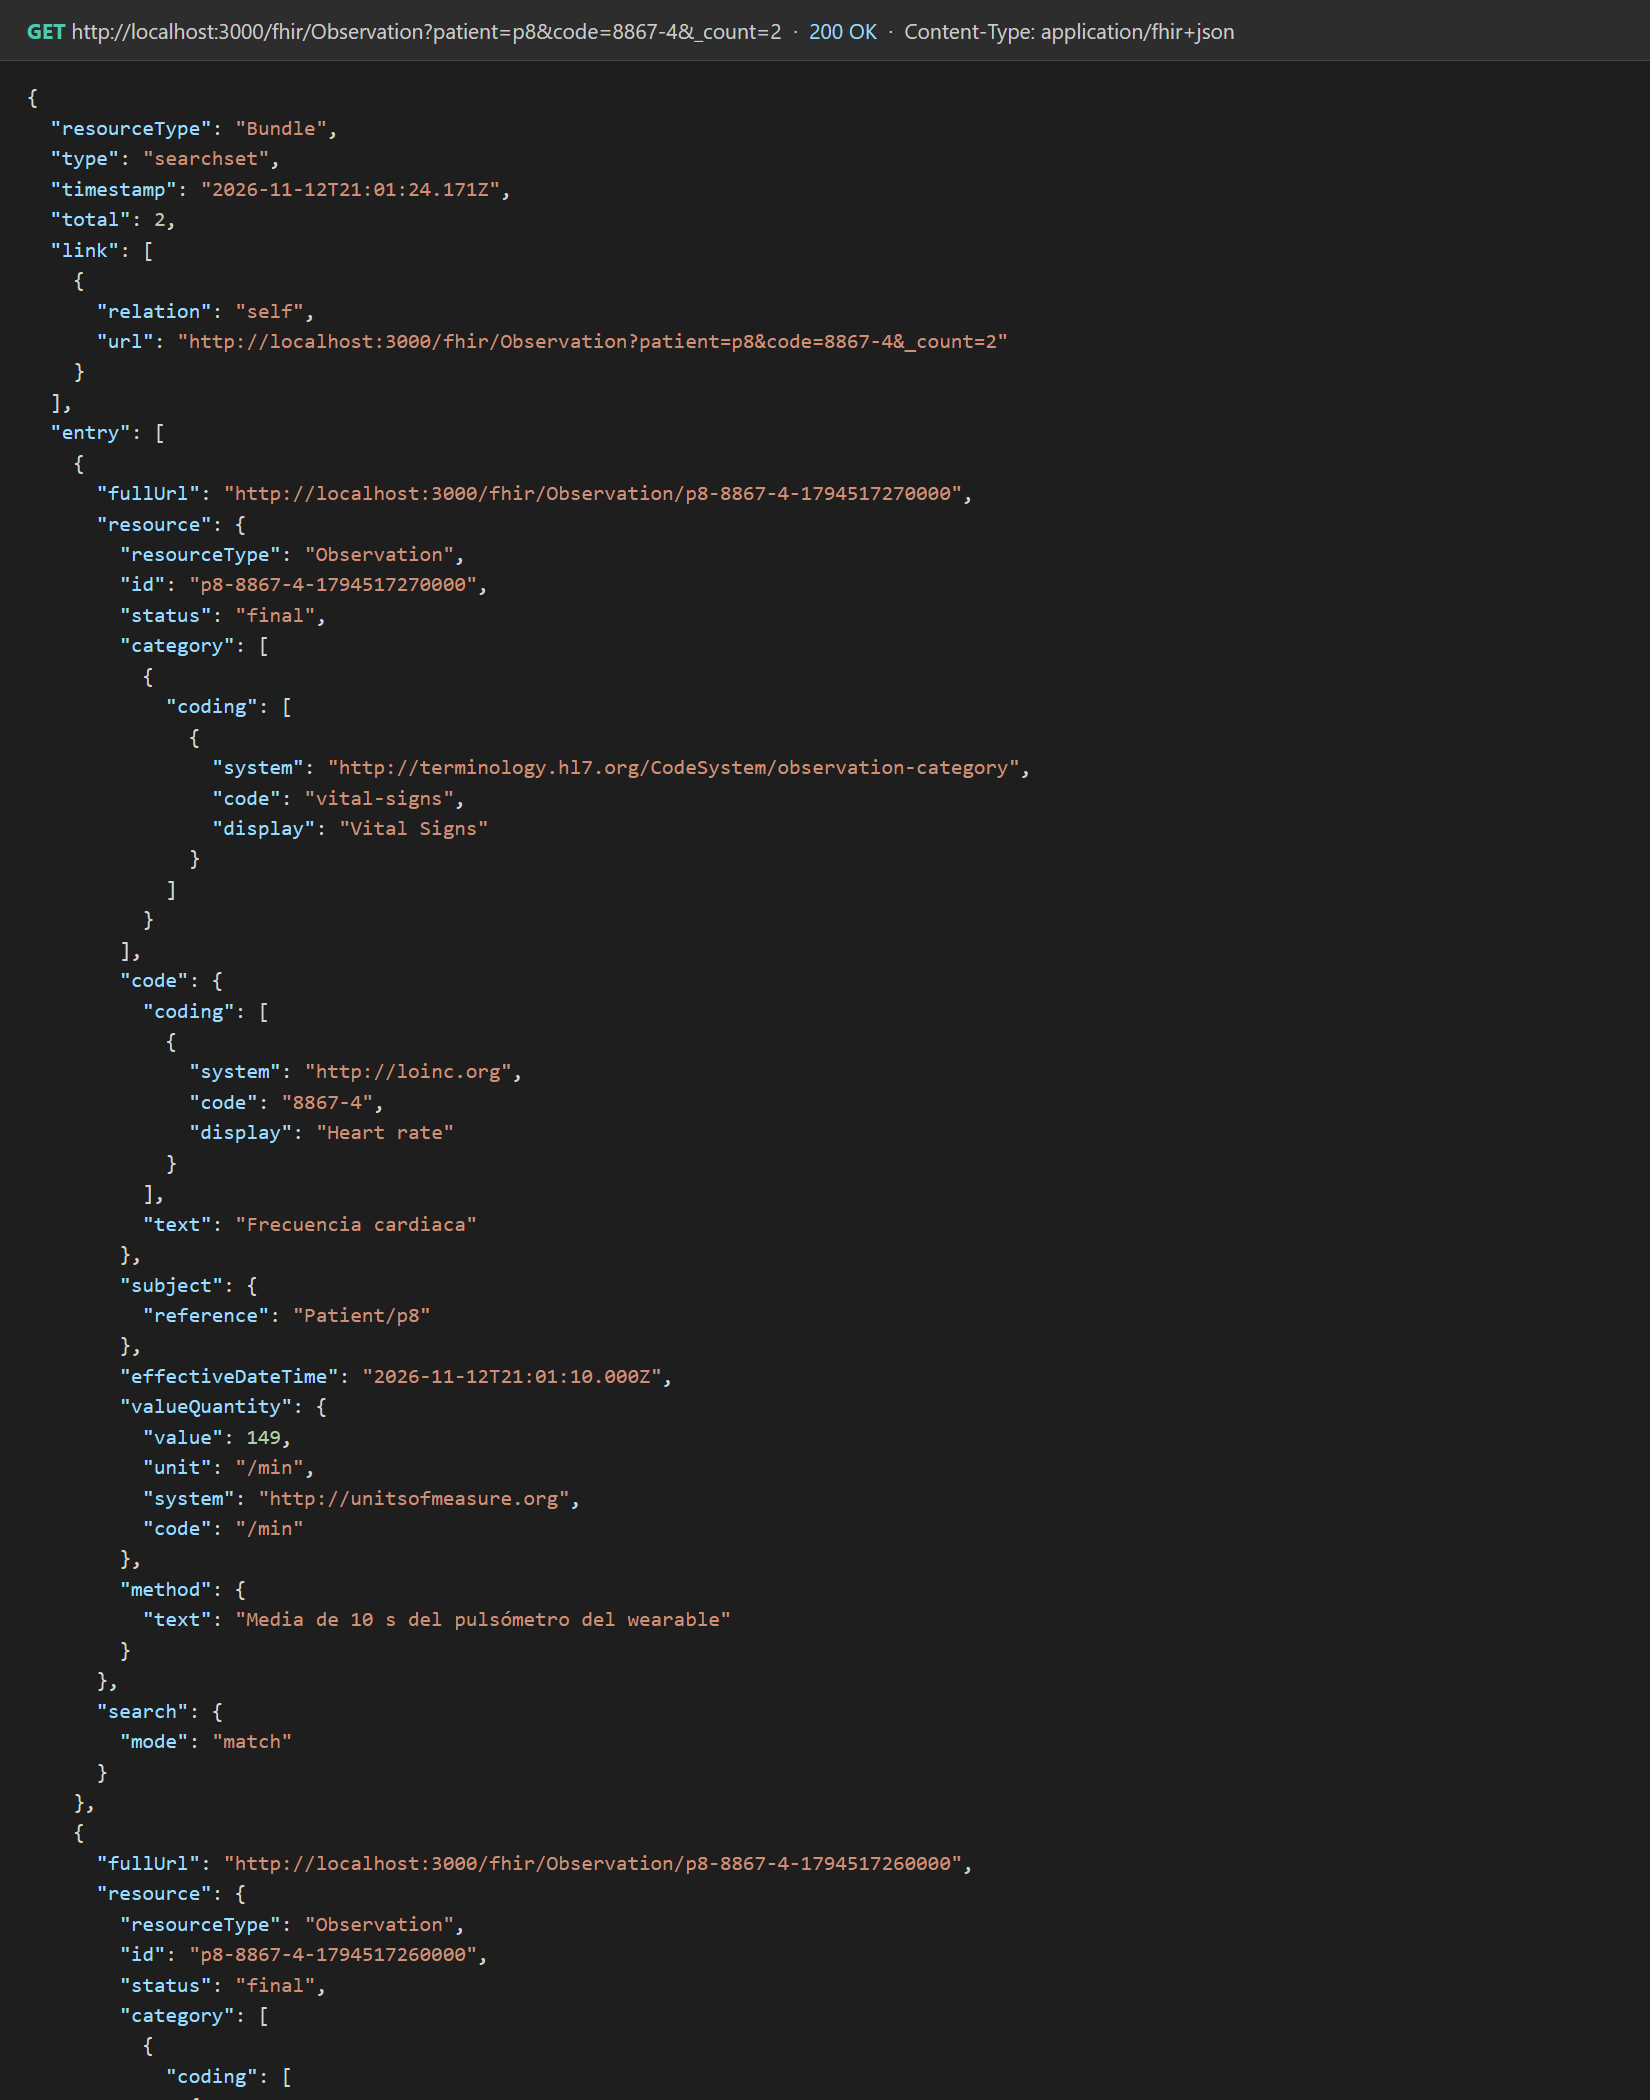
\includegraphics[width=0.6\textwidth]{fhir.png}
\caption{Respuesta de \texttt{/fhir/Observation}: un \texttt{Bundle} con \texttt{Observation} de frecuencia cardiaca (LOINC 8867-4).}
\label{fig:fhir}
\end{figure}

%%%%%%%%%%%%%%%%%%%%%%%%%%%%%%%%%%%%%%%%%%%%%%%%%%%%%%%%%%%%%%%%%%%%%%%%%%%%%%
\section{Dashboards}\label{sec:dashboards}
%%%%%%%%%%%%%%%%%%%%%%%%%%%%%%%%%%%%%%%%%%%%%%%%%%%%%%%%%%%%%%%%%%%%%%%%%%%%%%

El sistema ofrece tres páginas web, servidas por la API en el puerto 3000 y enlazadas entre sí, con el mismo aspecto: para el cuerpo médico, un \emph{dashboard} desde el que se actúa y un campograma que muestra al equipo sobre el campo; y, para preparar la demostración, una botonera de simulación que fuerza valores en el simulador. Las tres son HTML, CSS y JavaScript sin librerías y leen de la API con \texttt{fetch} y \texttt{WebSocket}.

\subsection{Dashboard médico}

Disponible en \url{http://localhost:3000/medico.html} (\ruta{api/public/medico.html}; Fig.~\ref{fig:dashboard}). Al abrirla carga los perfiles (\texttt{GET /api/jugadores}) y las alertas activas (\texttt{GET /api/alertas?estado=activa}), y a partir de ahí se actualiza sola con el WebSocket: la telemetría llega cada segundo y cada alerta nueva aparece en el momento con un aviso (``ALERTA CRÍTICA'' si es crítica). Tiene cinco bloques:

\begin{itemize}
  \item \textbf{Médico ya identificado.} La página no pide nada: carga \ruta{/medico-config.js}, donde la API le da la clave y el nombre del médico del \texttt{.env} (\texttt{API\_KEY\_MEDICO} y \texttt{MEDICO\_NOMBRE}), y arriba a la derecha muestra con qué nombre firma. Así la demostración va seguida (ver Sección~\ref{sec:seguridad}).
  \item \textbf{Equipo.} Una tarjeta por jugador con su dorsal, posición, FC (y \% de la FCmáx), temperatura, velocidad y alertas activas, con el borde del color de su semáforo (gris si lleva más de 5~s sin señal). Al pulsar una tarjeta se selecciona el jugador.
  \item \textbf{Alertas activas.} Primero las críticas y, dentro de cada severidad, de la más reciente a la más antigua, con un botón \emph{Confirmar} y una nota opcional por alerta (\texttt{POST /api/alertas/:id/confirmar}) y, si la alerta tiene tratamiento, un botón \emph{Enfriar} o \emph{Reposo} (ver más abajo).
  \item \textbf{Jugador seleccionado.} Zona de FC, zona de velocidad, asimetría y alertas; dos medidores de \% de la FCmáx y temperatura interna con las bandas de los umbrales, y dos gráficas de los últimos 2 minutos, de FC y de temperatura, con las líneas de los umbrales; empiezan con los resúmenes de 10~s de la API (\texttt{GET /api/jugadores/:id/historico}) y siguen con la telemetría en vivo.
  \item \textbf{Pauta de readaptación.} La pauta activa del jugador y un formulario para crear una nueva (velocidad máxima, carga máxima, asimetría máxima, vigencia y notas), que hace \texttt{POST /api/jugadores/:id/pauta}.
\end{itemize}

\textbf{El médico actúa y se ve el cambio.} Confirmar una alerta solo deja constancia de que el médico la ha visto. Para las alertas que dependen de un sensor que el simulador puede cambiar, el médico tiene además una intervención (\texttt{POST /api/alertas/:id/intervenir}, \ruta{services/intervenciones.js}):

\begin{itemize}
  \item \textbf{Enfriar} (\texttt{CALOR\_AMBAR}, \texttt{CALOR\_ROJA}): la temperatura baja paso a paso hasta 37,5~$^\circ$C. Imita el tratamiento del golpe de calor por esfuerzo, que es enfriar en el sitio con agua fría antes de trasladar al jugador; en la realidad se enfría a unos 0,15--0,35~$^\circ$C por minuto y se para hacia los 38,9~$^\circ$C \cite{nata2015}, y en la demo se comprime a unos 40~s.
  \item \textbf{Reposo} (\texttt{FC\_ALTA}, \texttt{FC\_DESACOPLE}, \texttt{RECUPERACION\_LENTA}, \texttt{INCIDENTE}): el pulso vuelve a 85~lpm.
\end{itemize}

La API publica ocho pasos, uno cada 5~s, por el mismo canal que la botonera (\topic{control/jugadores/<id>/sensores}), y al acabar quita el ajuste para que el simulador siga con sus valores normales. Mientras dura, la alerta aparece \emph{en tratamiento} con el valor de partida, el objetivo y el valor actual; al llegar, la API cierra sola las alertas de ese tipo del jugador con una nota que dice qué se hizo. En las gráficas, una línea azul discontinua marca cuándo se forzó el valor desde la botonera y una verde, cuándo intervino el médico, así que se ve la subida, la intervención y la bajada. \texttt{SOBRECARGA}, \texttt{ASIMETRIA}, \texttt{PAUTA\_EXCEDIDA} y \texttt{SIN\_SENAL} no dependen de un valor que el simulador pueda forzar: se confirman con una nota (y, para la carga, con una pauta).

\begin{figure}[!htbp]
\centering
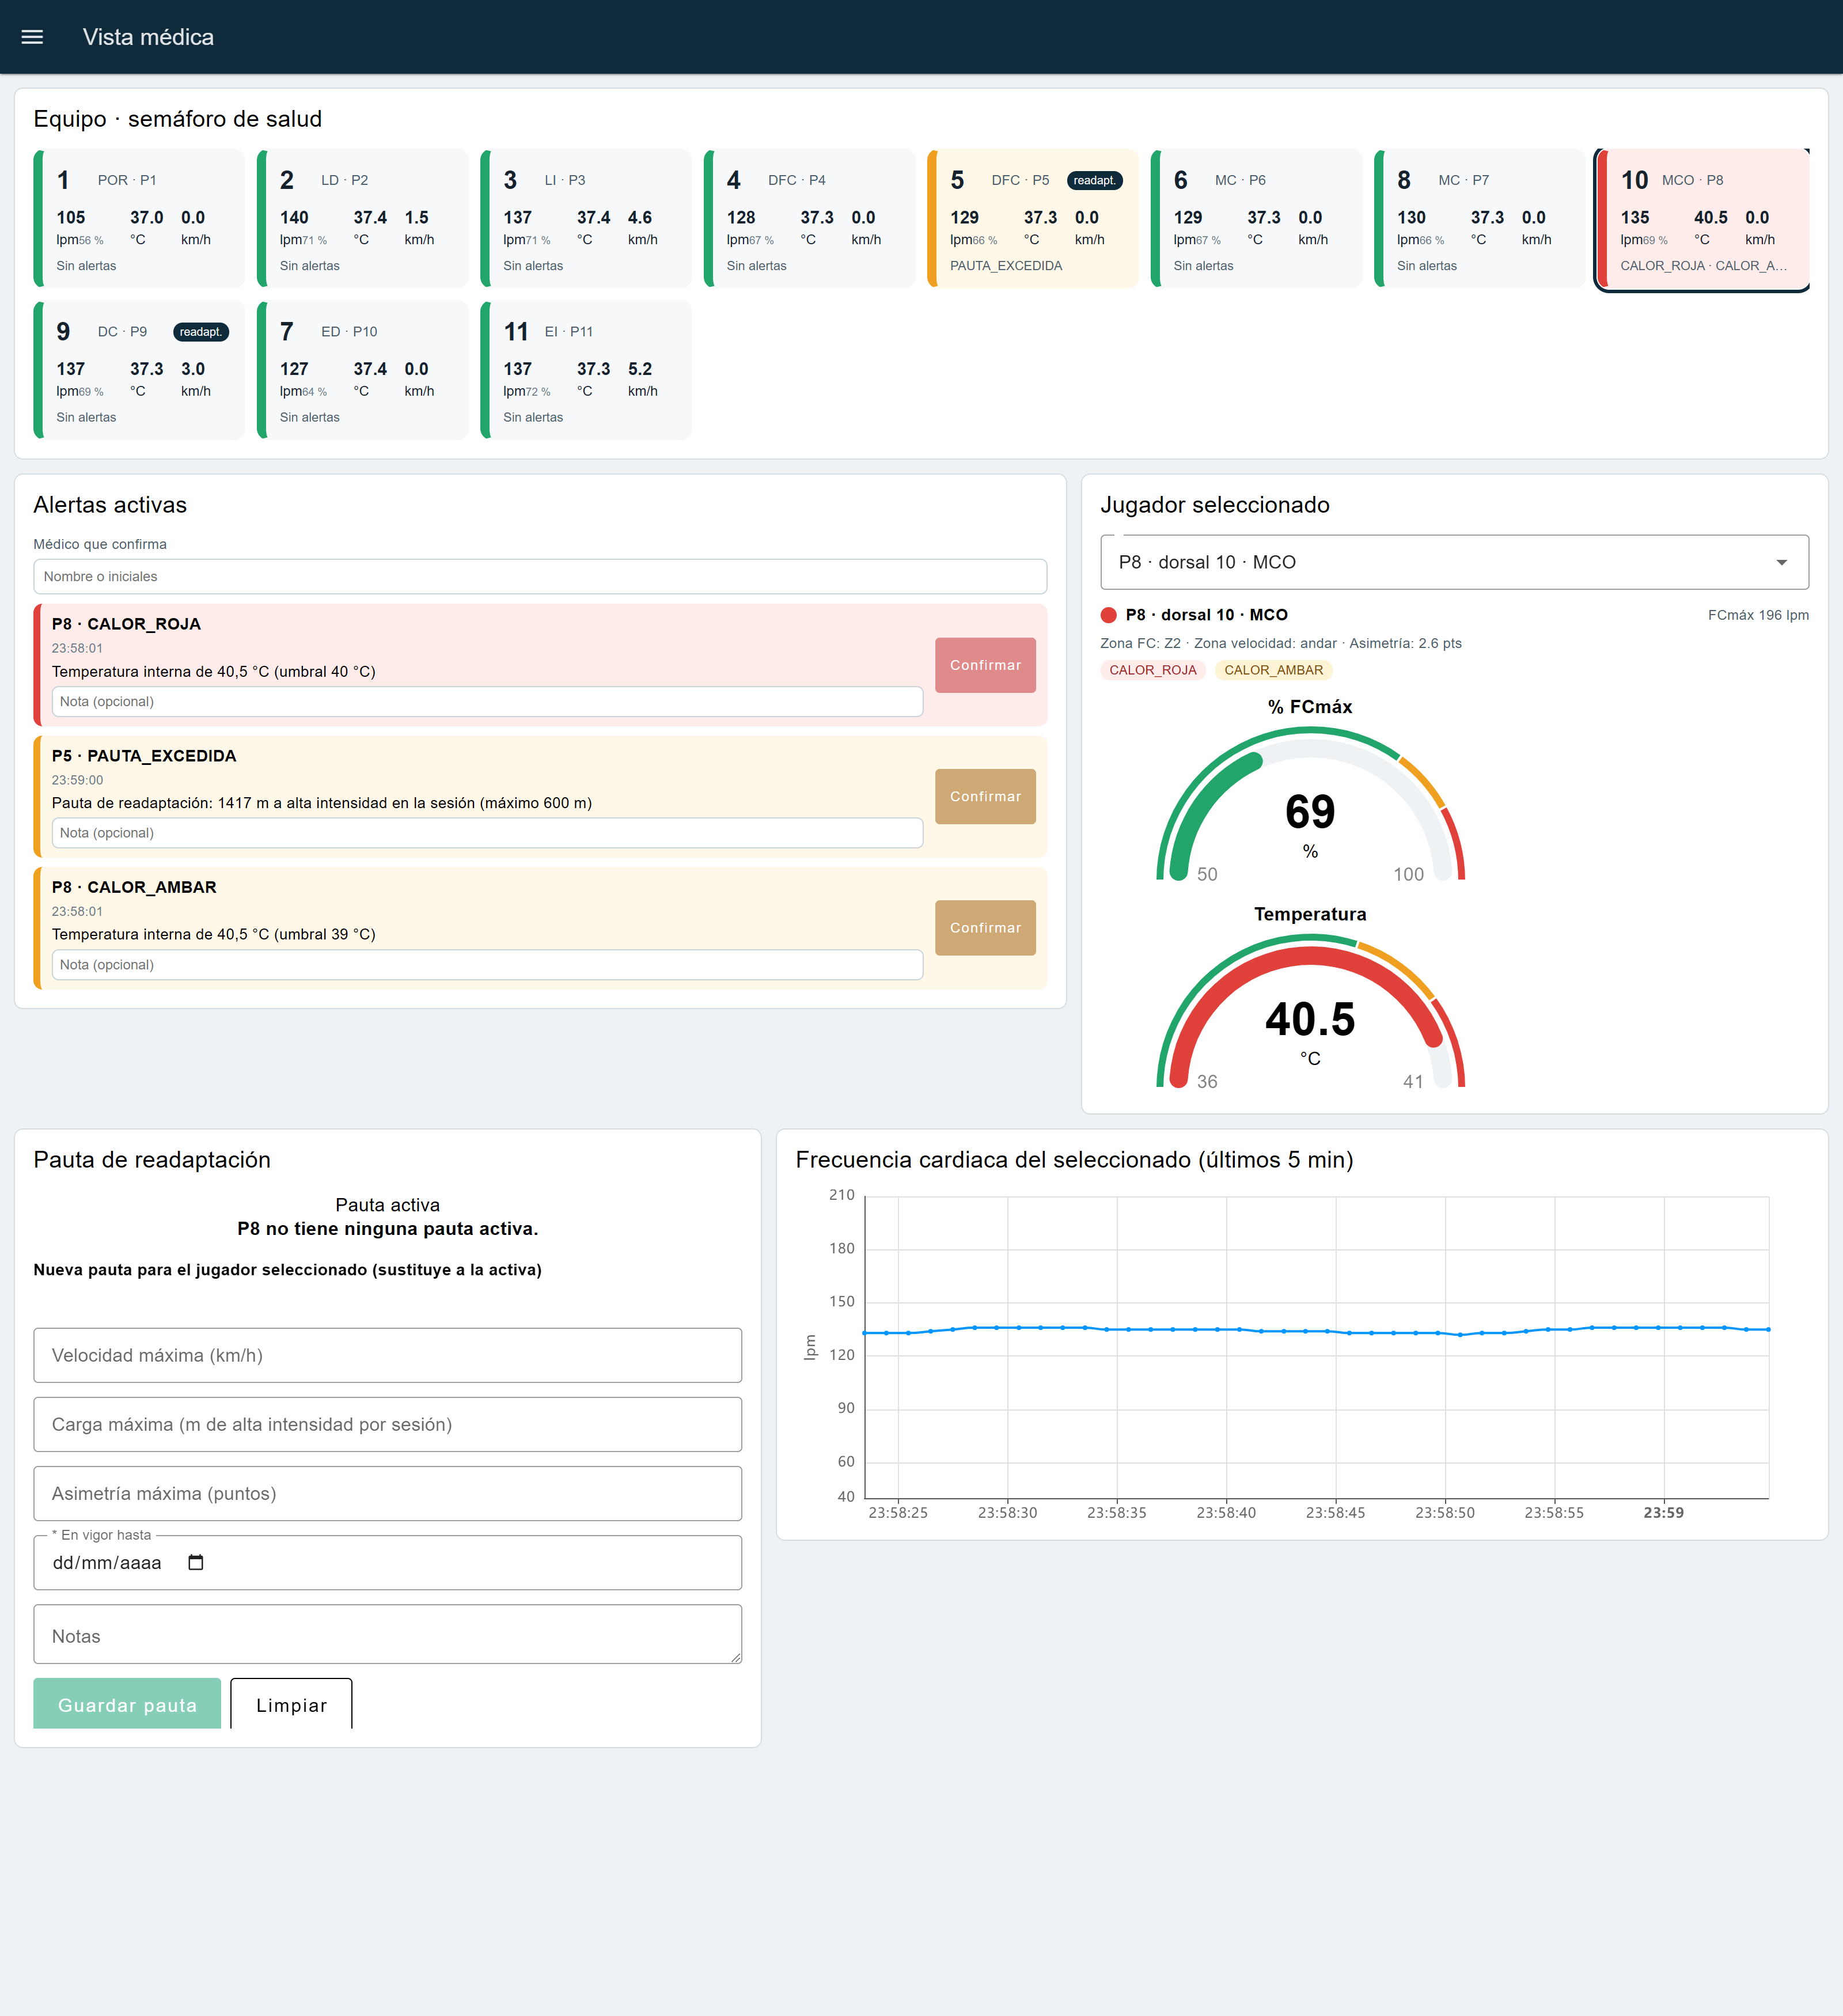
\includegraphics[width=0.8\textwidth]{dashboard-medico.png}
\caption{Dashboard médico durante un golpe de calor provocado en P8 (dorsal 8): su tarjeta está en rojo y el resto del equipo en verde. Sus dos alertas de calor esperan a que el médico pulse \emph{Enfriar} o \emph{Confirmar}; a la derecha, la ficha de P8 con la temperatura disparada. Arriba, el nombre con el que firma el médico.}
\label{fig:dashboard}
\end{figure}

\subsection{Campograma web}

La API sirve en \url{http://localhost:3000} una web propia (\ruta{api/public/index.html}), diseñada a partir de un prototipo de la parte de simulación y conectada a la API con \texttt{fetch} y \texttt{WebSocket} (Fig.~\ref{fig:campograma}). Muestra:

\begin{itemize}
  \item el campo con los once jugadores moviéndose en tiempo real, cada uno con el color de su línea y su dorsal; un aro ámbar indica un aviso y un aro rojo que late, una alerta crítica; el balón, la fase de juego y la posesión;
  \item el resumen del equipo: jugadores con señal, velocidad media, distancia total y alertas activas, y a quién se le está forzando un valor desde el simulador;
  \item la ficha del jugador seleccionado: velocidad, FC, distancia, posición, temperatura interna, curva de velocidad, reparto de carga entre pies, aceleraciones, giro y sus alertas activas.
\end{itemize}

La página solo lee: no guarda ninguna clave, y las alertas se confirman desde el \emph{dashboard} médico.

\begin{figure}[!htbp]
\centering
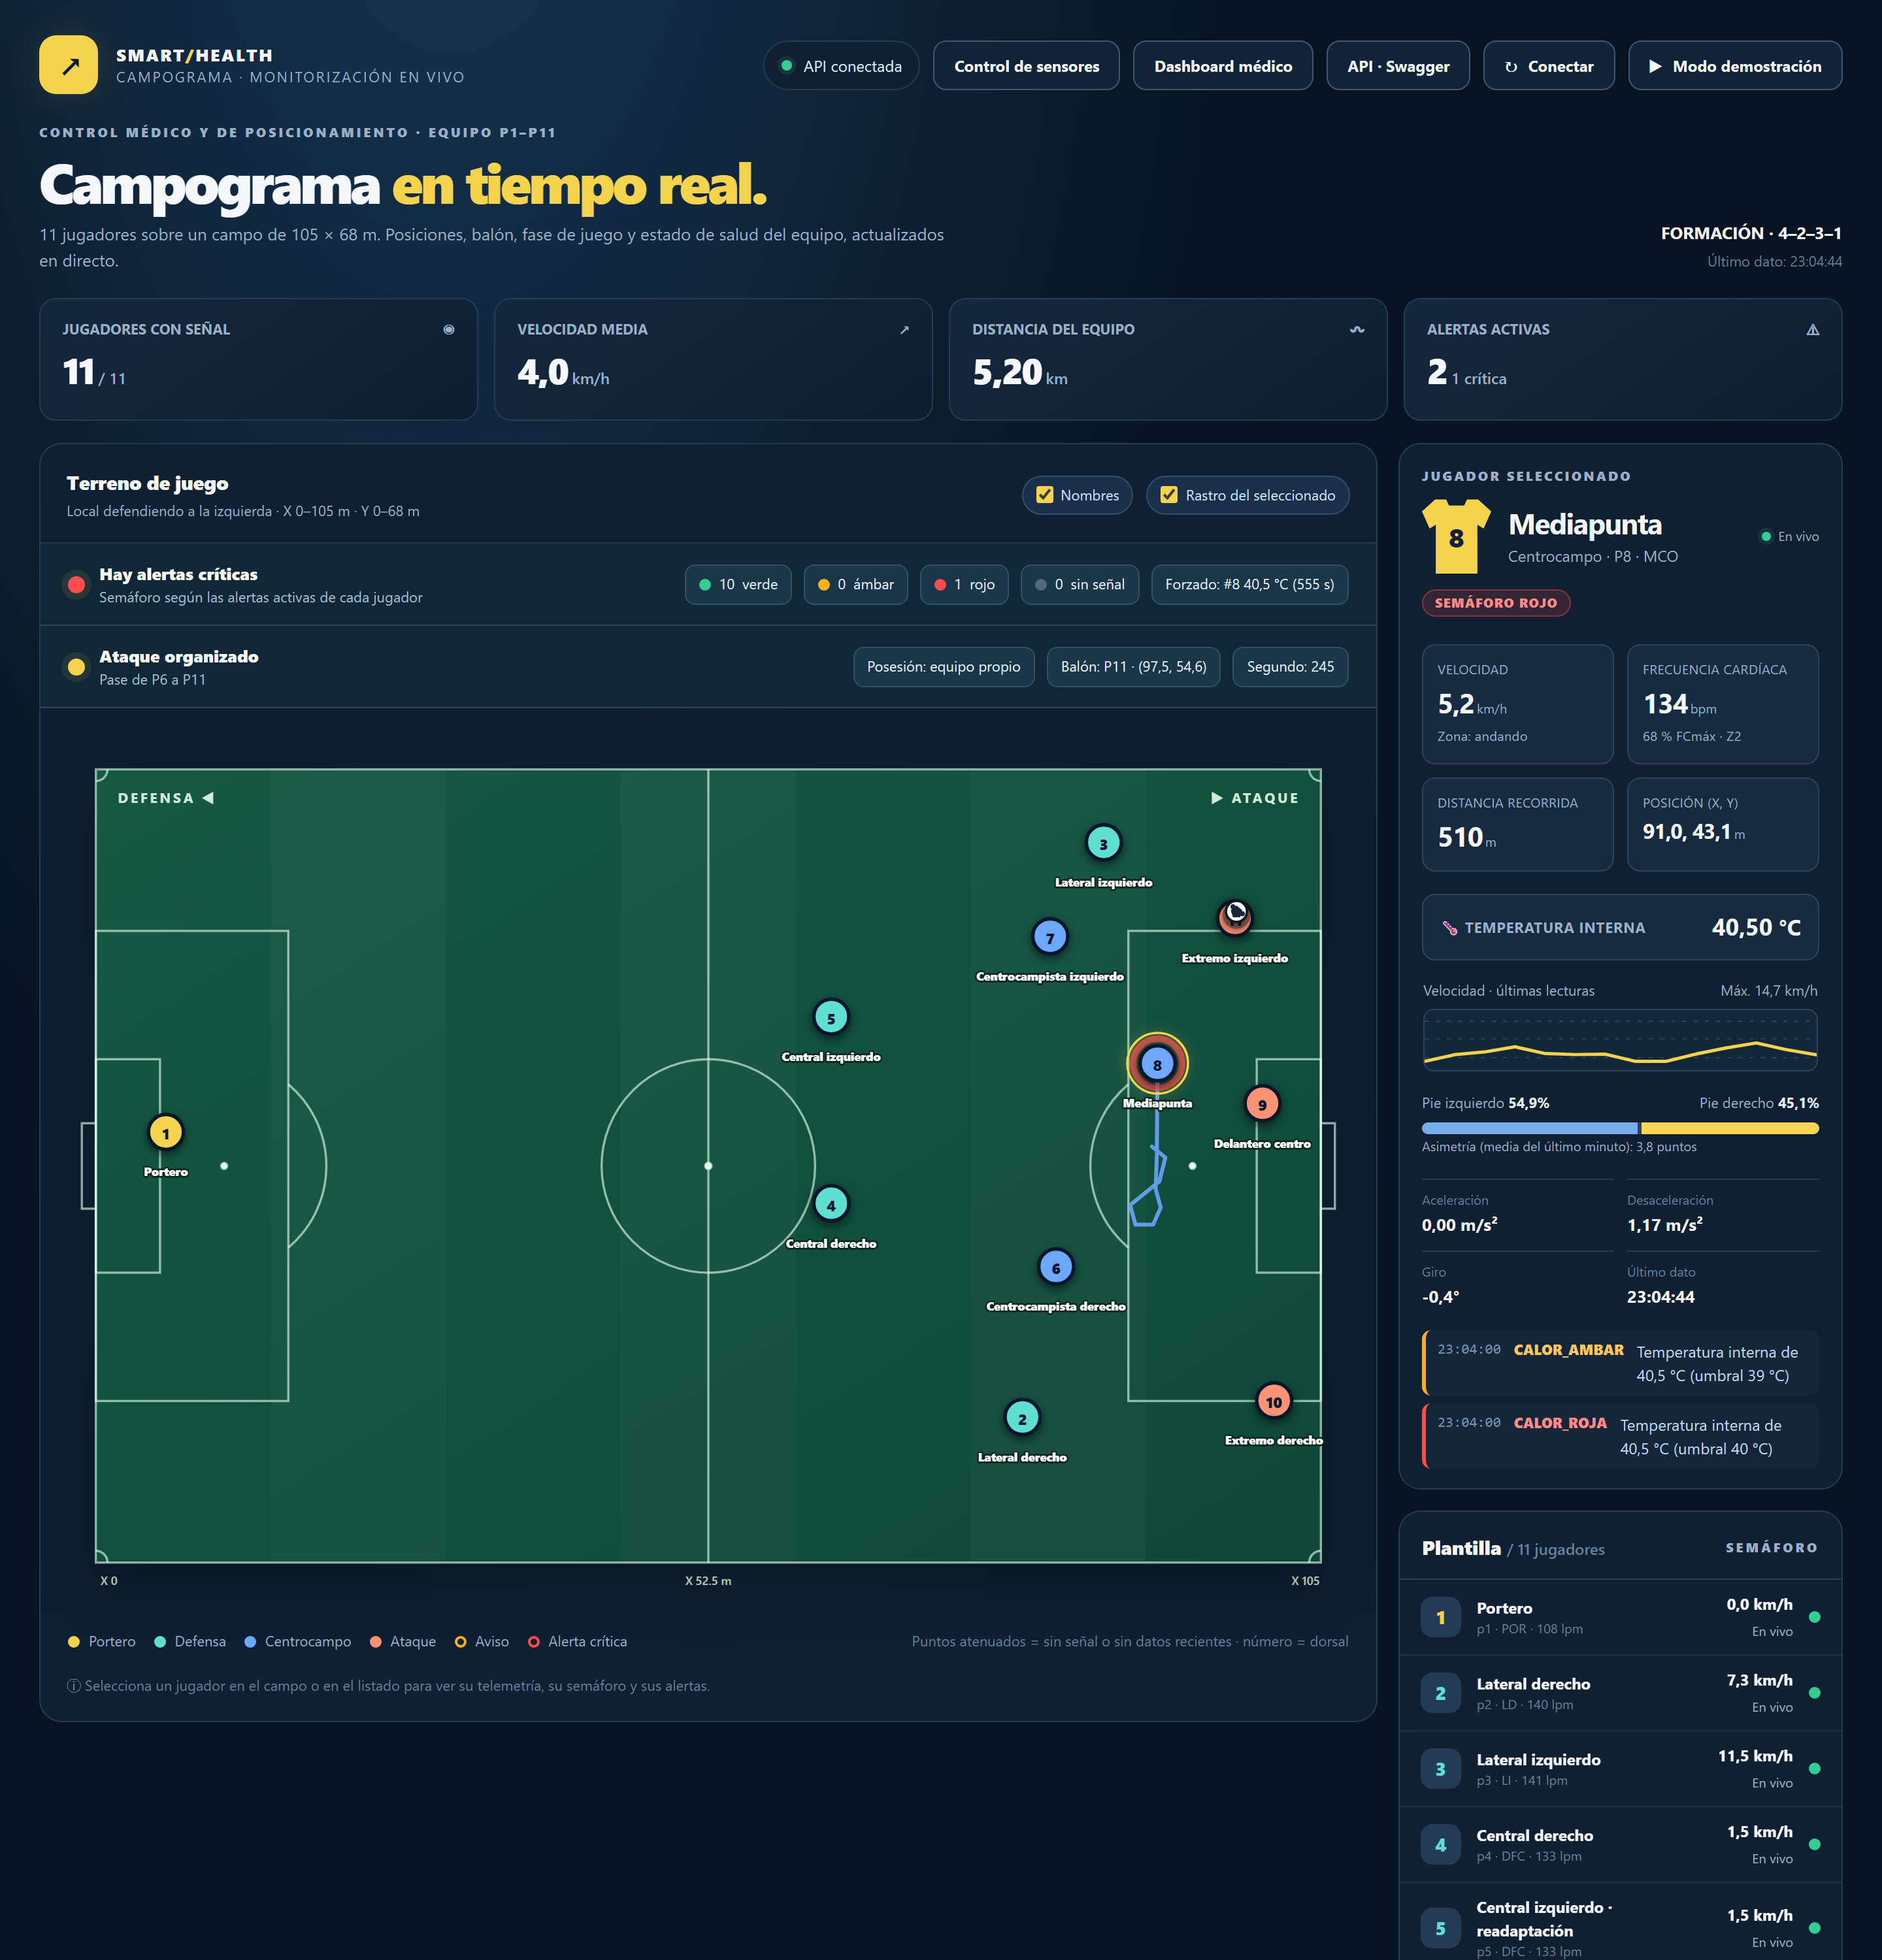
\includegraphics[width=0.92\textwidth]{campograma-alerta.png}
\caption{Campograma con una alerta crítica: el aro del dorsal 8 (p8) late en rojo, el panel indica ``Forzado: \#8 40,5~$^\circ$C'' y la ficha del jugador muestra sus dos alertas de calor.}
\label{fig:campograma}
\end{figure}

\subsection{Botonera de simulación}\label{sec:botonera}

Para provocar los escenarios de la demostración sin escribir peticiones a mano, la API sirve una segunda página en \url{http://localhost:3000/control.html} (\ruta{api/public/control.html}, enlazada desde el campograma; Fig.~\ref{fig:botonera}). Es el \emph{dashboard} de simulación y solo usa las rutas de \ruta{/api/simulador}:

\begin{itemize}
  \item se elige el jugador (P1--P11) y la duración del ajuste (1--3600~s, o ``hasta que lo retire'', que envía \texttt{durationSeconds: 0});
  \item botones rápidos de temperatura (37; 39,2 y 40,5~$^\circ$C) y de pulso (45, 150 y 195~lpm), un valor a medida para cada uno (35--42~$^\circ$C y 30--220~lpm, los rangos de la API) y ``Forzar ambos'', que hacen \texttt{PUT /api/simulador/jugadores/:id/sensores};
  \item ``Retirar ajustes'', que hace \texttt{DELETE} sobre esa ruta, y cinco botones de fase de juego (\texttt{POST /api/simulador/fase});
  \item las lecturas de temperatura y pulso que llegan del jugador por el WebSocket, la última orden que recuerda la API y un historial de las peticiones de la sesión.
\end{itemize}

Una respuesta \texttt{202} solo indica que la orden se publicó en el broker; por eso la página enseña al lado la lectura que vuelve del simulador, que es la confirmación real. Como las rutas del simulador, no pide clave ni toca datos clínicos.

\begin{figure}[!htbp]
\centering
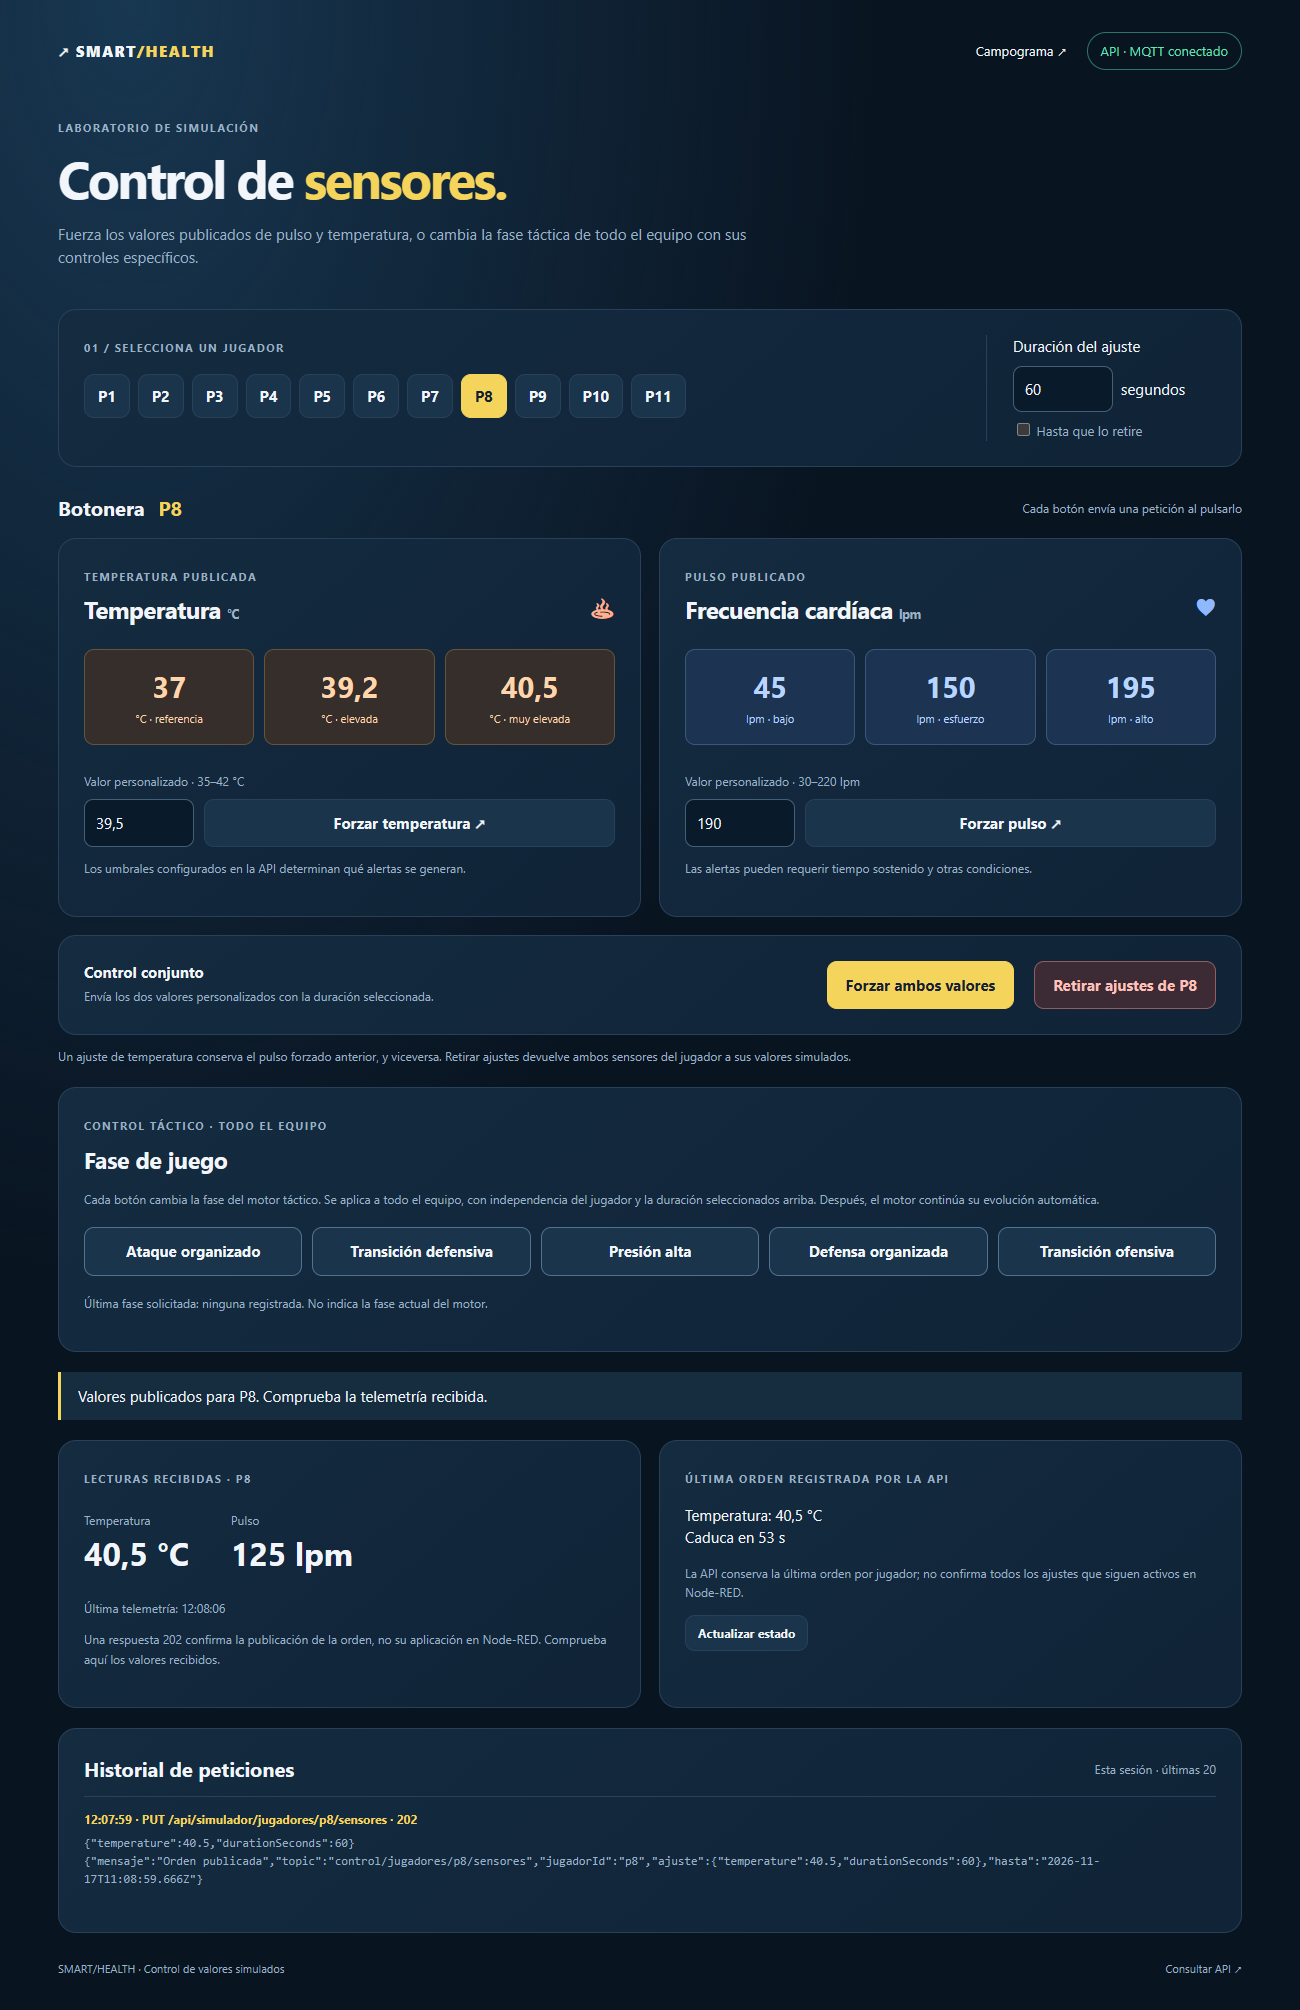
\includegraphics[width=0.68\textwidth]{botonera.png}
\caption{Botonera de simulación: se ha forzado 40,5~$^\circ$C a P8 y la tarjeta de lecturas confirma que el simulador ya publica ese valor.}
\label{fig:botonera}
\end{figure}

%%%%%%%%%%%%%%%%%%%%%%%%%%%%%%%%%%%%%%%%%%%%%%%%%%%%%%%%%%%%%%%%%%%%%%%%%%%%%%
\section{Privacidad y seguridad}\label{sec:seguridad}
%%%%%%%%%%%%%%%%%%%%%%%%%%%%%%%%%%%%%%%%%%%%%%%%%%%%%%%%%%%%%%%%%%%%%%%%%%%%%%

La frecuencia cardiaca, la temperatura interna, las lesiones y las pautas son \textbf{datos de salud}, una categoría especial según el artículo~9 del RGPD \cite{rgpd}. Las medidas adoptadas son:

\begin{itemize}
  \item \textbf{Seudonimización y minimización.} Los jugadores se identifican solo con \texttt{p1}\ldots\texttt{p11}, en los topics MQTT y en la base de datos; no se guarda ningún nombre. Se guardan resúmenes de 10~s y no la señal completa.
  \item \textbf{Broker cerrado.} Mosquitto no admite conexiones anónimas; cada cliente tiene usuario y contraseña, y la ACL aplica mínimo privilegio: la API solo puede escribir alertas y órdenes al simulador, y no puede leer nada; Node-RED solo puede leer \topic{control/\#}.
  \item \textbf{Autenticación por API key con dos roles} (cabecera \texttt{x-api-key}, \ruta{middleware/clave.js}): la clave de la pasarela solo puede enviar telemetría; la del médico es la única que escribe datos clínicos. Una clave válida usada en una operación que no le corresponde recibe \texttt{403}. Las claves se comparan en tiempo constante (\texttt{crypto.timingSafeEqual} sobre su \emph{hash} SHA-256).
  \item \textbf{Secretos fuera del repositorio.} Claves de la API y contraseñas de Mosquitto en el \texttt{.env} (incluido en \texttt{.gitignore}); en los flujos de Node-RED solo aparecen variables de entorno.
  \item \textbf{La clave del médico no está en el código de la web.} No aparece en ningún fichero de \ruta{api/public/}: la API la lee del \texttt{.env} y se la da al \emph{dashboard} médico en \ruta{/medico-config.js} (sin caché), que la envía en la cabecera \texttt{x-api-key}. Se precarga para que la demostración sea fluida; a cambio, quien pueda abrir \ruta{/medico.html} actúa como médico, por lo que esa página no se comparte fuera de la red de confianza (en la defensa, el túnel público solo se usa para la botonera). Sin \texttt{API\_KEY\_MEDICO} la página queda en solo lectura.
  \item \textbf{Validación estricta de la entrada} (tipos, unidades, rangos y tamaño del lote) y errores sin detalles internos.
\end{itemize}

\textbf{Limitaciones conocidas.} Es un entorno de desarrollo: los \texttt{GET} no piden clave, no hay HTTPS ni TLS en MQTT, las claves son por rol y no por usuario, la del médico va precargada en su página y no hay límite de peticiones. En producción harían falta HTTPS y MQTT sobre TLS, autenticación por usuario (por ejemplo OAuth~2.0 / OpenID Connect), clave también para leer, registro de accesos y cifrado de la base de datos.

%%%%%%%%%%%%%%%%%%%%%%%%%%%%%%%%%%%%%%%%%%%%%%%%%%%%%%%%%%%%%%%%%%%%%%%%%%%%%%
\section{Pruebas y demostración}
%%%%%%%%%%%%%%%%%%%%%%%%%%%%%%%%%%%%%%%%%%%%%%%%%%%%%%%%%%%%%%%%%%%%%%%%%%%%%%

\subsection{Pruebas realizadas}

\begin{itemize}
  \item \textbf{Tests automáticos:} 69 tests con \texttt{node:test} (\texttt{npm test}) sobre las partes puras: validación del lote, estado en vivo y resúmenes de 10~s, métricas, las diez reglas y el antirrebote, ACWR, conversión a FHIR, estado táctico, validación de las órdenes al simulador y la configuración del \emph{dashboard} médico. Todos pasan.
  \item \textbf{Colección de Postman:} las 47 peticiones pasan con el \emph{Collection Runner}, incluidos los errores esperados (400, 401, 403, 404 y 409).
  \item \textbf{Broker:} una conexión sin usuario se rechaza (\texttt{not authorised}); el usuario \texttt{nodered} recibe cada orden de \ruta{/api/simulador} sin denegaciones de la ACL.
  \item \textbf{Integración con el simulador:} un partido de 90 minutos (356.400 mensajes, 5.400 lotes) pasó por la pasarela, la validación y el motor de alertas sin ningún lote rechazado. Esta prueba destapó los dos ajustes de calibración; después, tres partidos de dos horas sin alertas falsas.
  \item \textbf{De extremo a extremo:} Mosquitto con usuarios y ACL $\rightarrow$ simulador y pasarela en Node-RED $\rightarrow$ API $\rightarrow$ MongoDB $\rightarrow$ \emph{dashboard} y campograma, con \texttt{/health} indicando MongoDB y MQTT conectados.
  \item \textbf{Prueba en limpio:} el repositorio se clonó desde GitHub en otro equipo y arrancó siguiendo solo el README.
\end{itemize}

\subsection{Guion de la demostración}

El vídeo sigue el escenario que motiva el proyecto:

\begin{enumerate}
  \item Partido normal: los once jugadores en verde en el campograma y en el \emph{dashboard}.
  \item Se provoca un golpe de calor a p8 desde la botonera de simulación (botón 40,5~$^\circ$C), que hace \texttt{PUT /api/simulador/jugadores/p8/sensores}.
  \item En unos segundos saltan \texttt{CALOR\_AMBAR} y \texttt{CALOR\_ROJA}: notificación en el \emph{dashboard}, tarjeta en rojo y aro rojo en el campograma (Figs.~\ref{fig:dashboard} y~\ref{fig:campograma}).
  \item El médico pulsa \emph{Enfriar}: la temperatura de p8 baja en las gráficas y la alerta se cierra sola. Después le pone una pauta de readaptación; cuando el jugador la supera, salta \texttt{PAUTA\_EXCEDIDA}.
  \item Swagger, Postman y la respuesta FHIR.
\end{enumerate}

%%%%%%%%%%%%%%%%%%%%%%%%%%%%%%%%%%%%%%%%%%%%%%%%%%%%%%%%%%%%%%%%%%%%%%%%%%%%%%
\section{Conclusiones}
%%%%%%%%%%%%%%%%%%%%%%%%%%%%%%%%%%%%%%%%%%%%%%%%%%%%%%%%%%%%%%%%%%%%%%%%%%%%%%

Se ha construido una plataforma IoT completa que integra todas las piezas pedidas (servidor Express con API REST, broker Mosquitto con MQTT, varios flujos de Node-RED y un \emph{dashboard}) y añade WebSockets, base de datos, tres páginas web en tiempo real (\emph{dashboard} médico, campograma y botonera de simulación), el estándar FHIR y documentación OpenAPI con su colección de Postman.

Las principales lecciones del trabajo son:

\begin{itemize}
  \item \textbf{Los contratos permiten trabajar en paralelo.} Fijar al principio los topics, los payloads y la API permitió que cada miembro avanzara en su bloque; cuando el formato del simulador cambió, bastó con actualizar el contrato a la versión 2.0.
  \item \textbf{Cada protocolo en su sitio.} MQTT para muchos mensajes pequeños y frecuentes, REST para consultar y modificar, y WebSocket para empujar el tiempo real al navegador.
  \item \textbf{Simular bien obliga a calibrar.} Conectar el motor de alertas a un simulador realista destapó falsos positivos que los tests unitarios no veían, y se corrigieron con medidas.
  \item \textbf{Los datos de salud exigen diseño desde el principio:} seudónimos, minimización, mínimo privilegio en el broker y roles en la API.
\end{itemize}

\textbf{Trabajo futuro.} Sustituir la simulación por \emph{wearables} reales; añadir HTTPS, MQTT sobre TLS y autenticación por usuario; publicar un acelerómetro con impacto para que la regla \texttt{INCIDENTE} pueda saltar con el simulador; un \emph{dashboard} de simulación propio en Node-RED; y gráficas históricas y de ACWR en el \emph{dashboard} médico.

%%%%%%%%%%%%%%%%%%%%%%%%%%%%%%%%%%%%%%%%%%%%%%%%%%%%%%%%%%%%%%%%%%%%%%%%%%%%%%
\begin{thebibliography}{10}
%%%%%%%%%%%%%%%%%%%%%%%%%%%%%%%%%%%%%%%%%%%%%%%%%%%%%%%%%%%%%%%%%%%%%%%%%%%%%%

\bibitem{buller2013}
Buller, M.J., Tharion, W.J., Cheuvront, S.N., et al.: Estimation of human core temperature from sequential heart rate observations. Physiological Measurement \textbf{34}(7), 781--798 (2013)

\bibitem{cole1999}
Cole, C.R., Blackstone, E.H., Pashkow, F.J., Snader, C.E., Lauer, M.S.: Heart-rate recovery immediately after exercise as a predictor of mortality. New England Journal of Medicine \textbf{341}(18), 1351--1357 (1999). \url{https://pubmed.ncbi.nlm.nih.gov/10536127/}

\bibitem{gabbett2016}
Gabbett, T.J.: The training-injury prevention paradox: should athletes be training smarter and harder? British Journal of Sports Medicine \textbf{50}(5), 273--280 (2016)

\bibitem{impellizzeri2020}
Impellizzeri, F.M., Tenan, M.S., Kempton, T., Novak, A., Coutts, A.J.: Acute:chronic workload ratio: conceptual issues and fundamental pitfalls. International Journal of Sports Physiology and Performance \textbf{15}(6), 907--913 (2020)

\bibitem{fhir}
HL7 International: FHIR R4, recurso Observation. \url{https://hl7.org/fhir/R4/observation.html}. Códigos LOINC: \url{https://loinc.org}

\bibitem{plantillas}
Plantillas instrumentadas y asimetría de carga. \url{https://pmc.ncbi.nlm.nih.gov/articles/PMC9208063}

\bibitem{nata2015}
Casa, D.J., DeMartini, J.K., Bergeron, M.F., et al.: National Athletic Trainers' Association position statement: exertional heat illnesses. Journal of Athletic Training \textbf{50}(9), 986--1000 (2015)

\bibitem{rgpd}
Reglamento (UE) 2016/679 del Parlamento Europeo y del Consejo (Reglamento General de Protección de Datos), artículo 9: tratamiento de categorías especiales de datos personales.

\bibitem{scisports}
SciSports: Physical variables glossary. \url{https://support.scisports.com/en/articles/4476826-physical-variables-glossary}

\bibitem{statsports}
STATSports: Maximum accelerations and decelerations: significance for an athlete's physical development. \url{https://statsports.com/the-locker/maximum-acceleration-and-decelerations-significance-for-an-athletes-physical-development}

\bibitem{tempfutbol}
Temperatura interna de futbolistas en partidos con calor. Journal of Science and Medicine in Sport (2025). \url{https://opus.lib.uts.edu.au/bitstream/10453/191965/2/PIIS1440244025005377.pdf}

\bibitem{tempreview}
Core body temperature responses during competitive sporting events: a narrative review. Biology of Sport. \url{https://www.termedia.pl/Core-body-temperature-responses-during-competitive-sporting-events-a-narrative-review,78,50091,1,1.html}

\end{thebibliography}

%%%%%%%%%%%%%%%%%%%%%%%%%%%%%%%%%%%%%%%%%%%%%%%%%%%%%%%%%%%%%%%%%%%%%%%%%%%%%%
\appendix
\section{Material entregado}
%%%%%%%%%%%%%%%%%%%%%%%%%%%%%%%%%%%%%%%%%%%%%%%%%%%%%%%%%%%%%%%%%%%%%%%%%%%%%%

\begin{itemize}
  \item \textbf{Código fuente} (incluidos los flujos de Node-RED): \texttt{PracticalAssignment2627\_GarciaDelgadoDeMendozaManuel\_SanzHuertaAlejandro.zip}.
  \item \textbf{Vídeo de demostración} (5 minutos): \pendiente{enlace de YouTube pendiente}.
  \item \textbf{Vídeo de TikTok} (opcional): \pendiente{enlace de TikTok pendiente}.
  \item \textbf{Documentación de la API:} Sección~\ref{sec:api} de este informe, Swagger UI en \texttt{/api-docs} (\ruta{api/openapi.yaml}), colección de Postman (\ruta{docs/postman\_collection.json}) y contratos en \ruta{docs/contratos/}.
\end{itemize}

\begin{table}[!htbp]
\centering
\caption{Estructura del repositorio.}\label{tab:repo}
\footnotesize
\begin{tabularx}{\textwidth}{p{3.6cm}L}
\toprule
\textbf{Carpeta} & \textbf{Contenido} \\
\midrule
\ruta{api/} & API REST en Express, WebSocket, modelos de Mongoose, motor de alertas y tests \\
\ruta{api/public/} & Campograma (\url{http://localhost:3000}), \emph{dashboard} médico (\texttt{/medico.html}) y botonera de simulación (\texttt{/control.html}) \\
\ruta{node\_red/} & Flujos: simulador (\texttt{flows.json}) y pasarela (\texttt{flows\_pasarela.json}); lanzador \texttt{arrancar.js} \\
\ruta{mosquitto/} & Configuración del broker y ACL \\
\ruta{docs/} & Contratos, diagramas y colección de Postman \\
\ruta{arrancar-todo.cmd} & Lanzador de todo el sistema en Windows Terminal \\
\bottomrule
\end{tabularx}
\end{table}

%%%%%%%%%%%%%%%%%%%%%%%%%%%%%%%%%%%%%%%%%%%%%%%%%%%%%%%%%%%%%%%%%%%%%%%%%%%%%%
\section{Cómo ejecutarlo}
%%%%%%%%%%%%%%%%%%%%%%%%%%%%%%%%%%%%%%%%%%%%%%%%%%%%%%%%%%%%%%%%%%%%%%%%%%%%%%

\textbf{Requisitos:} Node.js 24, Docker Desktop (solo para MongoDB), Mosquitto 2.1 y Node-RED 5.

\textbf{Arranque rápido.} En Windows, un doble clic en \texttt{arrancar-todo.cmd} abre Windows Terminal con una pestaña por pieza (Docker Desktop se abre antes a mano) y, cuando la API y Node-RED están listos, abre en el navegador el campograma, la botonera de simulación, el \emph{dashboard} médico y el editor de Node-RED. Cada arranque vacía la base de datos y carga los datos iniciales; con \texttt{-Conservar} no.

\textbf{Arranque paso a paso}, desde la raíz del repositorio:

\begin{lstlisting}[language=shell]
# 1. Variables de entorno: copiar .env.example como .env y rellenar claves y contraseñas
# 2. MongoDB
docker compose up -d
# 3. Mosquitto con la configuración del proyecto (consola de administrador)
net stop mosquitto
mosquitto -c mosquitto/mosquitto.conf -v
# 4. API (http://localhost:3000, Swagger en /api-docs)
cd api && npm install && npm run dev
# 5. Datos iniciales: los 11 jugadores (sin pautas: todos en verde)
cd api && npm run seed
# 6. Node-RED con los flujos del proyecto (editor en http://localhost:1880)
node node_red/arrancar.js
# Tests
cd api && npm test
\end{lstlisting}

\textbf{Direcciones:} campograma en \url{http://localhost:3000}, botonera de simulación en \url{http://localhost:3000/control.html}, Swagger en \url{http://localhost:3000/api-docs}, estado en \url{http://localhost:3000/health}, editor de Node-RED en \url{http://localhost:1880} y \emph{dashboard} médico en \url{http://localhost:3000/medico.html}.

\end{document}
